\documentclass[aps,preprint,floatfix,nofootinbib,showpacs]{revtex4-1}
\pdfoutput=1
\usepackage{amsmath}
\usepackage{amsfonts}
\usepackage{amssymb}
\usepackage{float}
\usepackage{color}
\usepackage{graphicx}
\usepackage{graphics}
%\usepackage{feynarts}
\usepackage{hyperref}
\hypersetup{ }
\usepackage{epstopdf}
\usepackage{adjustbox,lipsum}
%\usepackage{tgbonum}


\begin{document}

\title{Studying QCD Modeling uncertainties on particle spectra from dark matter annihilation into jets}
\date{\today}
\author{Simone Amoroso}
\affiliation{CERN, CH-1211, Geneva 23, Switzerland}
\author{Sasha Caron}
\affiliation{Nikhef, Science Park, Amsterdam, The Netherlands. \\
Institute of Physics, University of Amsterdam, Science Park 904, 1018 XE Amsterdam, The
Netherlands}
\author{Adil Jueid}
\affiliation{University AbdelMalek Essaadi, 
Facult\'e des Sciences et Techniques, D\'epartement de Math\'ematiques, 
B.P 416 Tangier, Morocco.}
\author{Roberto Ruiz de Austri}
\affiliation{Instituto de F\'isica Corpuscular, IFIC-UV/CSIC, Valencia, Spain}
\author{Peter Zeiler Skands}
\affiliation{School of Physics and Astronomy, Monash University, VIC-3800, Australia}

\begin{abstract}
Motivated by indirect searches for dark matter in the universe, we study the
uncertainties in the spectra of particles resulting from $e^+ e^-$ scattering in order
to constrain the spectra of $\gamma$ rays from dark matter annihilation. 
We investigate the uncertainties in some observables using
\texttt{PYTHIA} event generator at different center of mass energies. TO FOLLOW ...
\end{abstract}


\maketitle

%%%%%%%%%%%%%%%%%%%%%%%%%%%%%%%%%%%%%%%%%%%%%%%%%%%%%%%
\section{Introduction} %%%%%%%%%%%%%%%%%%%%%%%%%%%%%%%%
%%%%%%%%%%%%%%%%%%%%%%%%%%%%%%%%%%%%%%%%%%%%%%%%%%%%%%%
There is strong evidence suggesting that a mysterious “dark matter” exists which
accounts for about $22\%$ of the mass of the universe. Although the properties
of dark matter remain unknown, many models predict the annihilation of dark
matter into SM particles \cite{Bertone:2004pz}, e.g it could be annihilated 
to a quark anti-quark pair. On the other hand, those quarks will be radiating
additional quarks and gluons in form of showers and end up by fragmentating 
into color-neutral hadrons.
\begin{itemize}
 \item We have to discuss the rate of photons coming from the decay of those hadrons.
 \item Importance of the study of string fragmentation and shower uncertainties to constrain those spectra 
 and their role in the searches of dark matter from $\gamma$ rays ...
 \item Importance of modeling the bremsstrahlung photons as well..
 \item Any suggestions for other things to be included in the introduction ?
\end{itemize}

%%%%%%%%%%%%%%%%%%%%%%%%%%%%%%%%%%%%%%%%%%%%%%%%%%%%%%%
\section{Theory Models} %%%%%%%%%%%%%%%%%%%%%%%%%%%%%%%
%%%%%%%%%%%%%%%%%%%%%%%%%%%%%%%%%%%%%%%%%%%%%%%%%%%%%%%

%%%%%%%%%%%%%%%%%%%%%%%%%%%%%%%%%%%%%%%%%%%%%%%%%%%%%%%
\section{Setup} %%%%%%%%%%%%%%%%%%%%%%%%%%%%%%%%%%%%%%%
%%%%%%%%%%%%%%%%%%%%%%%%%%%%%%%%%%%%%%%%%%%%%%%%%%%%%%%
The first part of the uncertainties estimation is tuning of 
the parameters of the parton shower model and hadronization 
in Pythia to a set of sensitive LEP measurements. Our set
of theoretical predictions will be tuned against
\texttt{ALEPH} \cite{Barate:1996fi, Heister:2001jg, Heister:2001kp},
\texttt{DELPHI} \cite{Abreu:1996na, Abreu:1998nn, DELPHI_2002} and 
\texttt{OPAL} \cite{Akers:1994ez, Ackerstaff:1998ap, Abbiendi:2000cv} experiments.
In the first step, we will be tunig only the parameters of 
the light quark fragmentation function $a_L, b_L \text{ and } \sigma$ 
and consider 5 different tunes depending on included the observables:
\begin{itemize}
\item the manual tune denoted by \texttt{T1} where the parameters
are tuned manually against \texttt{L3}, and some of the distributions in \texttt{ALEPH}
using \texttt{Vincia} \cite{Giele:2007di}
 \item the second tune \texttt{T2} which includes mean particle multiplicities, event shapes, 
 scaled momentum distribution, jet rates, and some particle spectra. The included observables
 are shown in tables \ref{Tab1},\ref{Tab2},\ref{Tab3},\ref{Tab4}.
 \item the third tune denoted by \texttt{T3} includes only charged multiplicity, mean charged multiplicities,
 mean particle multiplicities ($\pi^0, \pi^\pm$), jet rates, scaled momentum distributions, and $\gamma, \pi^{0,\pm}, \eta$
 spectra. Tables \ref{Tab3} and \ref{Tab5} show the observables that we have included along with their 
 weights.
 \item \texttt{T4} denoting the fourth tune which includes scaled momentum distributions, mean pion multiplicities, 
 pion, photon and eta spectra and jet rates. The observables with their weights are shown in Tables \ref{Tab3} and \ref{Tab6}.
 \item finally, a fifth tune which uses $\pi^{0,\pm}, \gamma \text{ and } \eta$ to constrain the parameters. The weights
 are shown in \ref{Tab7}.
\end{itemize}
Except the first tune, all the other fits are performed using \texttt{Professor} \cite{Buckley:2009bj} with 
the analyses that are implemented in \texttt{Rivet} \cite{Buckley:2010ar}. We have 
chosen only the distributions that are sensitive to the variations 
of $a_L, b_L \text{ and } p_\perp(\sigma)$. The goodness of fit per 
degree-of-freedom is a measure of how well the MC predictions agree
with experiment. It is defined as follows:
\begin{eqnarray}
 \frac{\chi^2}{N_{df}} = \frac{\sum_{\mathcal{O}} 
 \omega_\mathcal{O} \sum_{b\in \mathcal{O}} (f_{(b)}(\textbf{p}) - \mathcal{R}_b)^2/\Delta_b^2}{\sum_{\mathcal{O}} \omega_\mathcal{O} |b \in \mathcal{O}|},
\label{Gof-Ndf}
 \end{eqnarray}
where $\mathcal{R}_b$ is the reference value and $\Delta_b$ is the total
experimental error of the data per bin and per distribution $\mathcal{O}$. The modeling
of the true MC response is done using a set of functions $f_{(b)}(\textbf{p})$. The weights
per observable and bin $\omega_\mathcal{O}$ are used to compute the goodness-of-fit. Furthermore,
the weights could have different values for different bins of the same observable. The functions
$f_{(b)}(\textbf{p})$ parameterising the MC response should be at least a polynomial of second-order.
We have been using a third-order polynomial to model the MC response, i.e:
\begin{eqnarray}
 f_{(b)}(\textbf{p}) = \alpha_0^{(b)} + \sum_i \beta_i^{(b)} p_i + \sum_{i \leq j} \gamma_{ij}^{(b)} q_i q_j +
 \sum_{i\leq j \leq k} \delta_{ijk} q_i q_j q_k,
 \label{MC-response}
\end{eqnarray}
with $\textbf{q} = \textbf{p} - \textbf{p}_0$ and $\textbf{p}_0$ is a reference point in the 
parameter space. We note, finally, that the modeling functions $f_{(b)}(\textbf{p})$ 
should be replaced by true MC functions $\text{MC}_{(b)}$ if real MC samples are used.
To get a good tune, we have to use a big number of MC runs. For this study, 110 random combinations
of 1000 runs have been used. 
The method of eigentunes in \texttt{Professor} is used to get an estimate of the 
uncertainty in the MC predictions where a change of the parameter values is 
performed. The paramters are changed in the eigenvectors directions where the 
eigenvectors are obtained by a change of in the goodness-of-fit (Gof) 
per number of degrees-of-freedom; 
$\Delta \chi^2/N_{df}$ in $\chi^2/N_{df}$ corresponding to the true minimization. 
For each parameter, two eigenvectors exist; one in the positive direction and the other 
in the negative direction. Furthermore, if $\chi^2/N_{df} \leq 1$ one-sigma deviation 
from the central tune is obtained for $\Delta \chi^2/N_{df} = 1$ and two-sigma deviation
for $\Delta \chi^2/N_{df} = 4$ and so on.
However, MC generators are not able to achieve $\Delta \chi^2/N_{df} \leq 1$. In this case,
the eigentunes could be used to have a rough estimate of the range of variations around
the central tune that event generators could achieve. Three sets of eigentunes have 
been computed with \texttt{Professor} corresponding to one-, two- and three-sigma deviations with 
respect to the central tune.

%%%%%%%%%%%%%%%%%%%%%%%%%%%%%%%%%%%%%%%%%%%%%%%%%%%%%%%
\section{Results}
%%%%%%%%%%%%%%%%%%%%%%%%%%%%%%%%%%%%%%%%%%%%%%%%%%%%%%%
\subsection{Results of the tunes}

 \begin{table}[!h]
  \begin{center}
   \begin{tabular}{l|l|l|l|l|l}
    \hline \hline
    Parameter  & \hspace{1cm} \texttt{T1} \hspace{0.5cm} & \hspace{1cm} \texttt{T2} \hspace{0.5cm} & \hspace{1cm} \texttt{T3} \hspace{0.5cm}& \hspace{1cm} \texttt{T4} \hspace{0.5cm} & \hspace{1cm} \texttt{T5} \hspace{0.5cm}  \\ \hline
    $a_L$      & \hspace{1cm} $0.8$  \hspace{0.5cm}    & \hspace{1cm} $0.967$ \hspace{0.5cm} & \hspace{1cm} $0.92$ \hspace{0.5cm} & \hspace{1cm} $0.9095$ \hspace{0.5cm} & \hspace{1cm} $0.7863$ \hspace{0.5cm} \\ \hline
    $b_L$      & \hspace{1cm} $1.13$ \hspace{0.5cm}     & \hspace{1cm}  $1.14$ \hspace{0.5cm} & \hspace{1cm} $1.06$ \hspace{0.5cm} & \hspace{1cm} $1.048$ \hspace{0.5cm} & \hspace{1cm} $0.6502$ \hspace{0.5cm} \\ \hline
    $p_\perp (\text{GeV})$  & \hspace{1cm} $0.327$ \hspace{0.5cm} & \hspace{1cm} $0.303176$ \hspace{0.5cm}  & \hspace{1cm} $0.3093$ \hspace{0.5cm} & \hspace{1cm} $0.3092$ \hspace{0.5cm} & \hspace{1cm} $0.3515$ \hspace{0.5cm}\\ \hline \hline
   \end{tabular}
  \end{center}
  \caption{Results of the different fits.}
  \label{Fit-1}
 \end{table}
 In Table \ref{Fit-1}, we show the minimization results of the different tunes. We can see 
 that \texttt{T2}, \texttt{T3} and \texttt{T4} give more or less the same results while
 \texttt{T1} and \texttt{T4} give higher values for $p_\perp$. We plot in Figs. \ref{Chi2-1}-\ref{Chi2-5}  the 
 $\chi^2$ values computed using \texttt{Vincia} of three observables; $x$, $\log(1/x_p)$ and charged multiplicity.
 We can see that \texttt{T1} give the best $\chi^2$ values. We note that the \texttt{Professor} tunes
 give reasonable agreement with data for event shapes.
 \begin{figure}[!h]
 \centering
 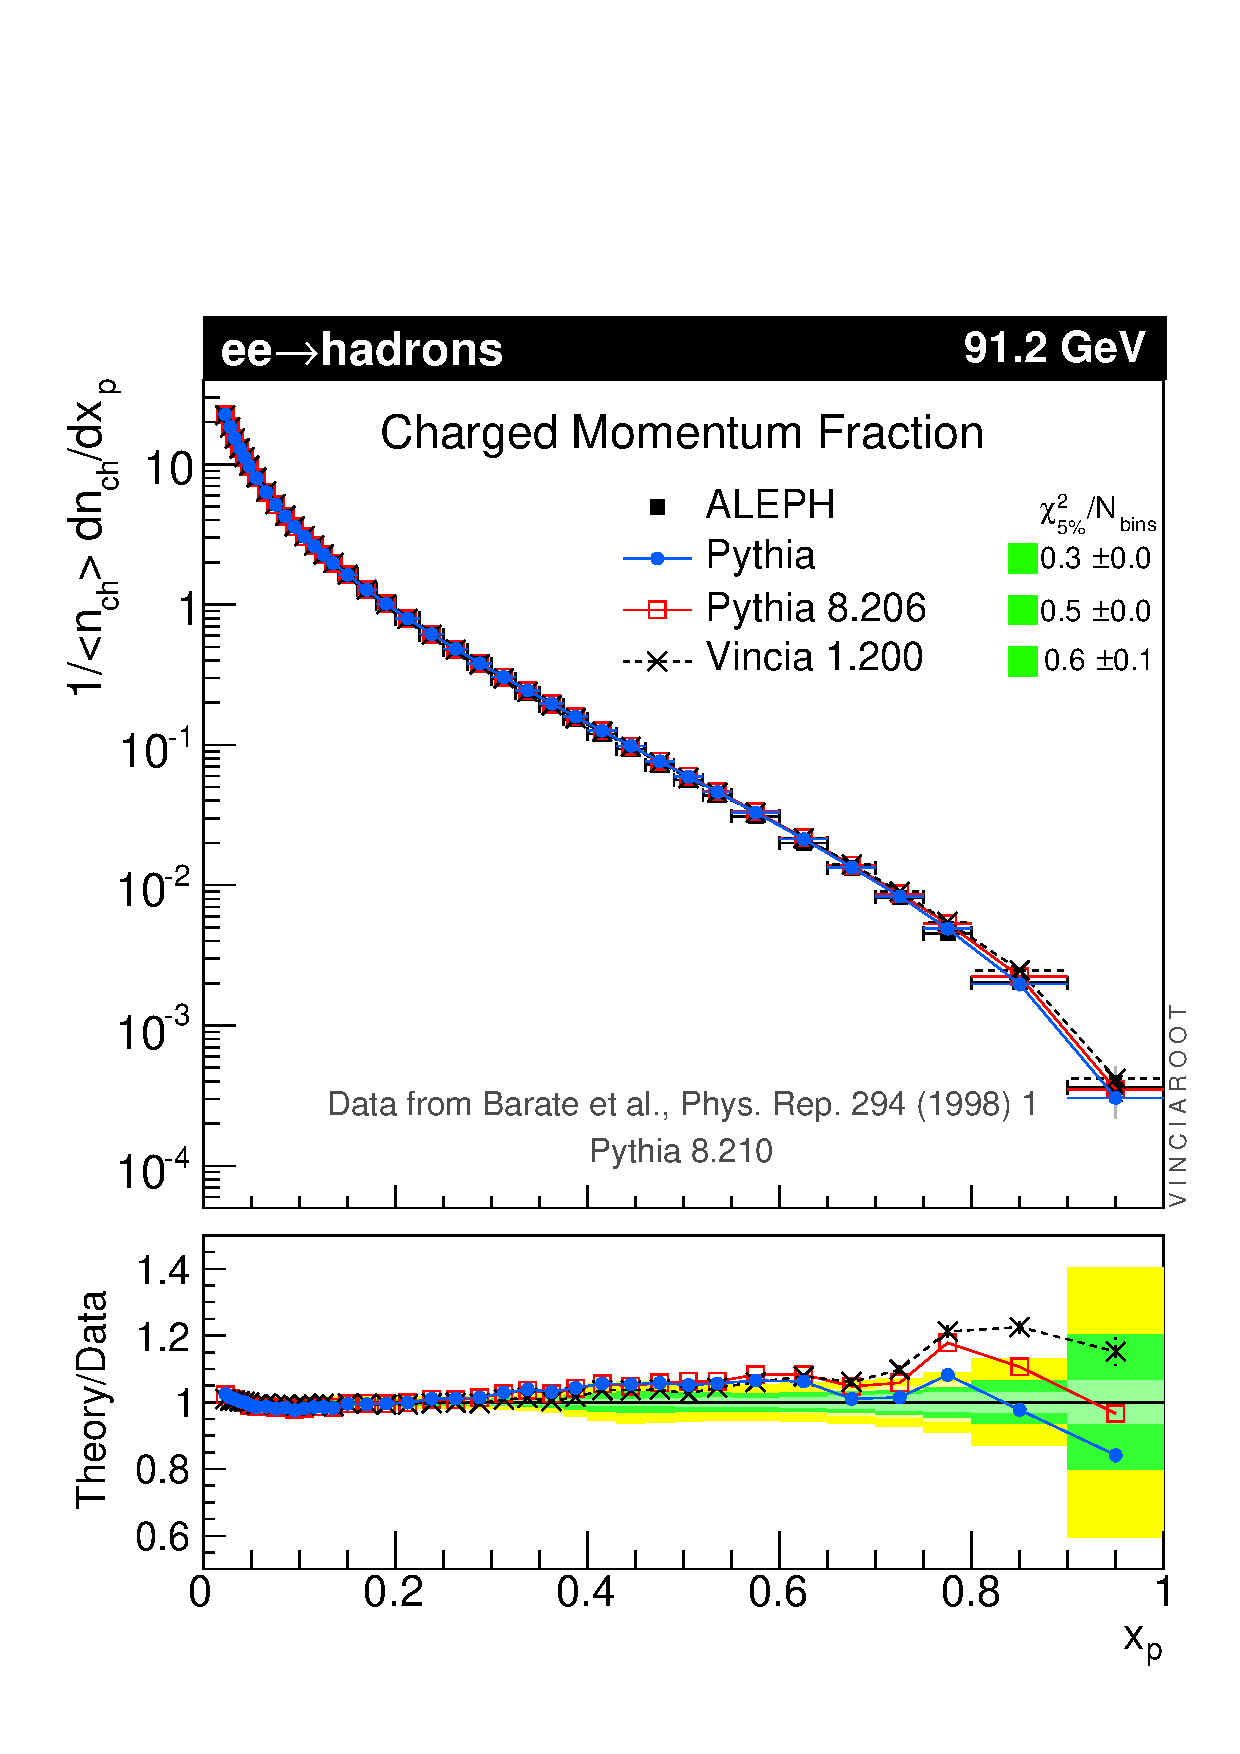
\includegraphics[width=5cm, height=5cm]{Vincia-T1/vincia03-x.pdf}
 \hfill
 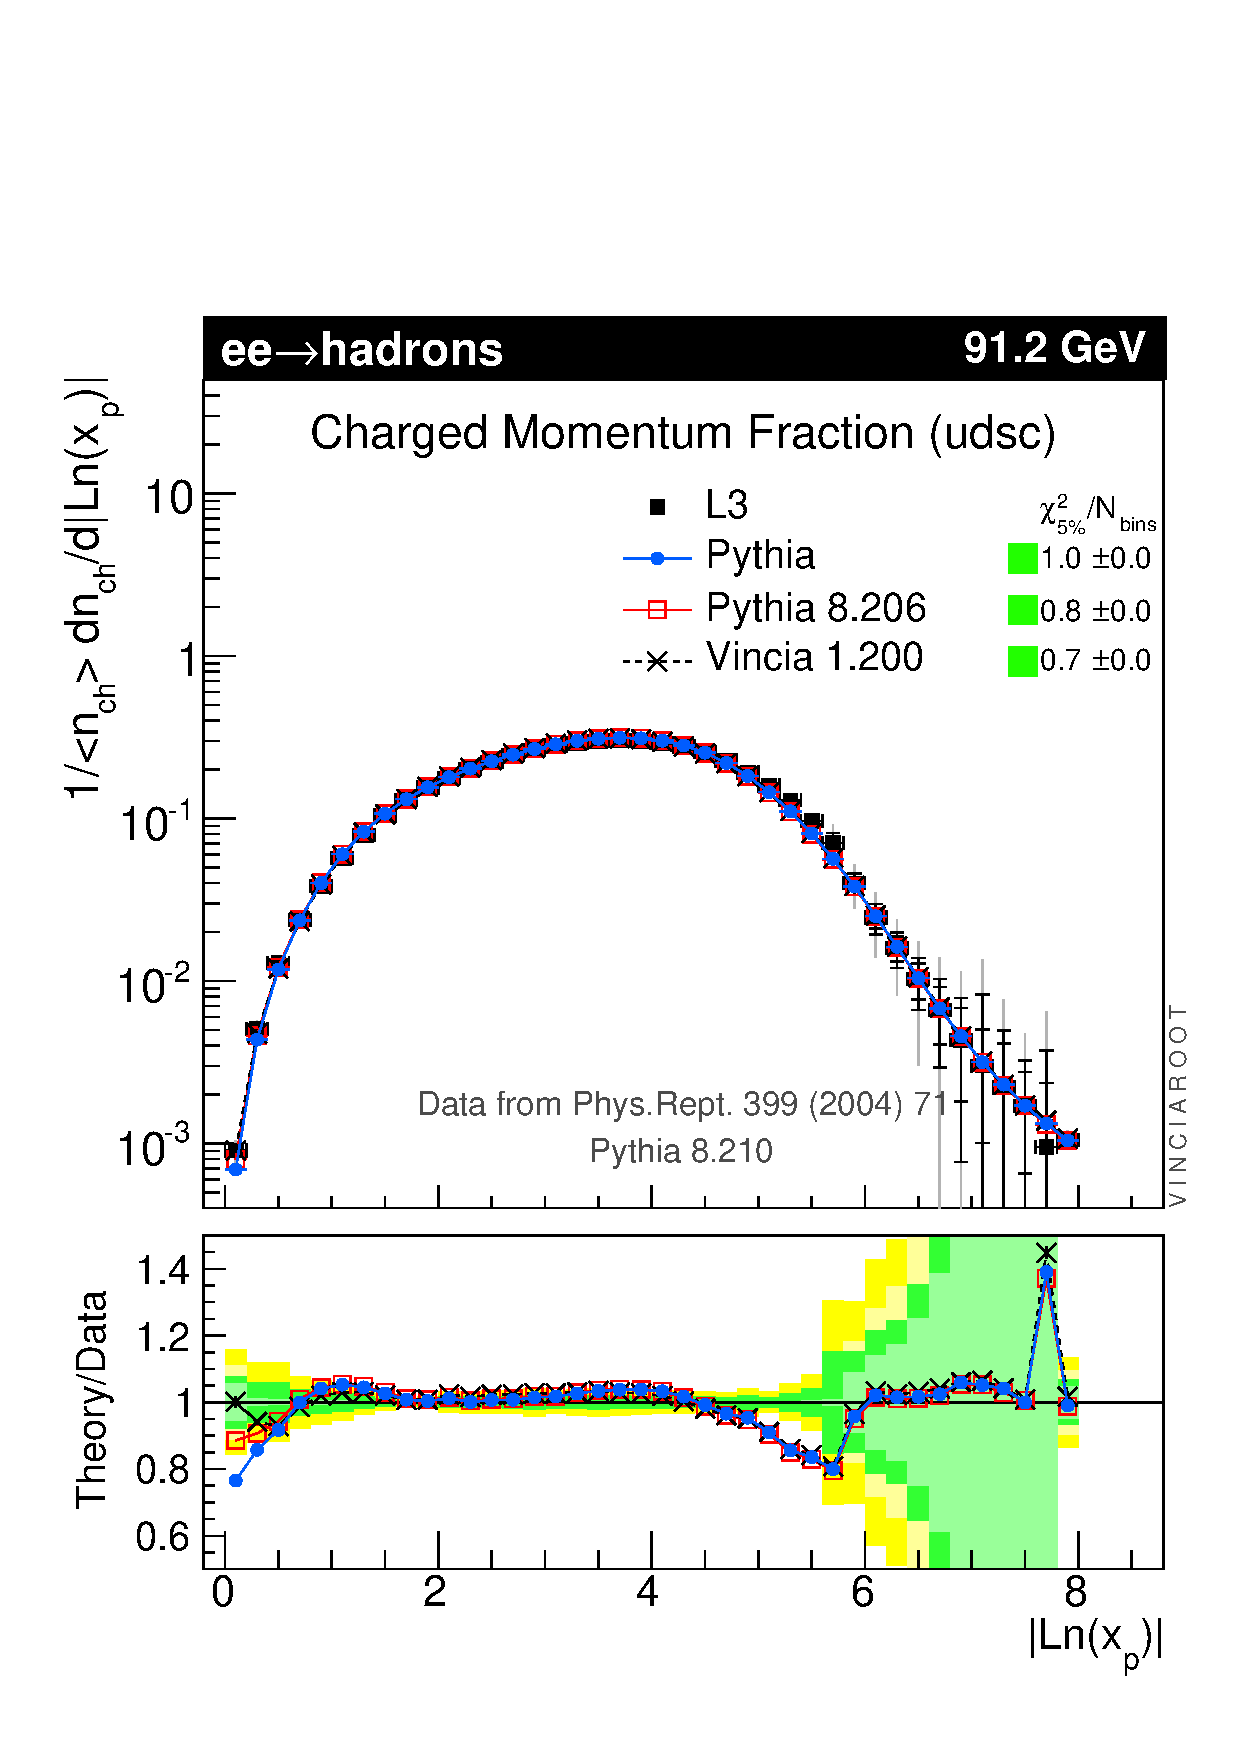
\includegraphics[width=5cm, height=5cm]{Vincia-T1/vincia03-Lnx.pdf}
 \hfill
 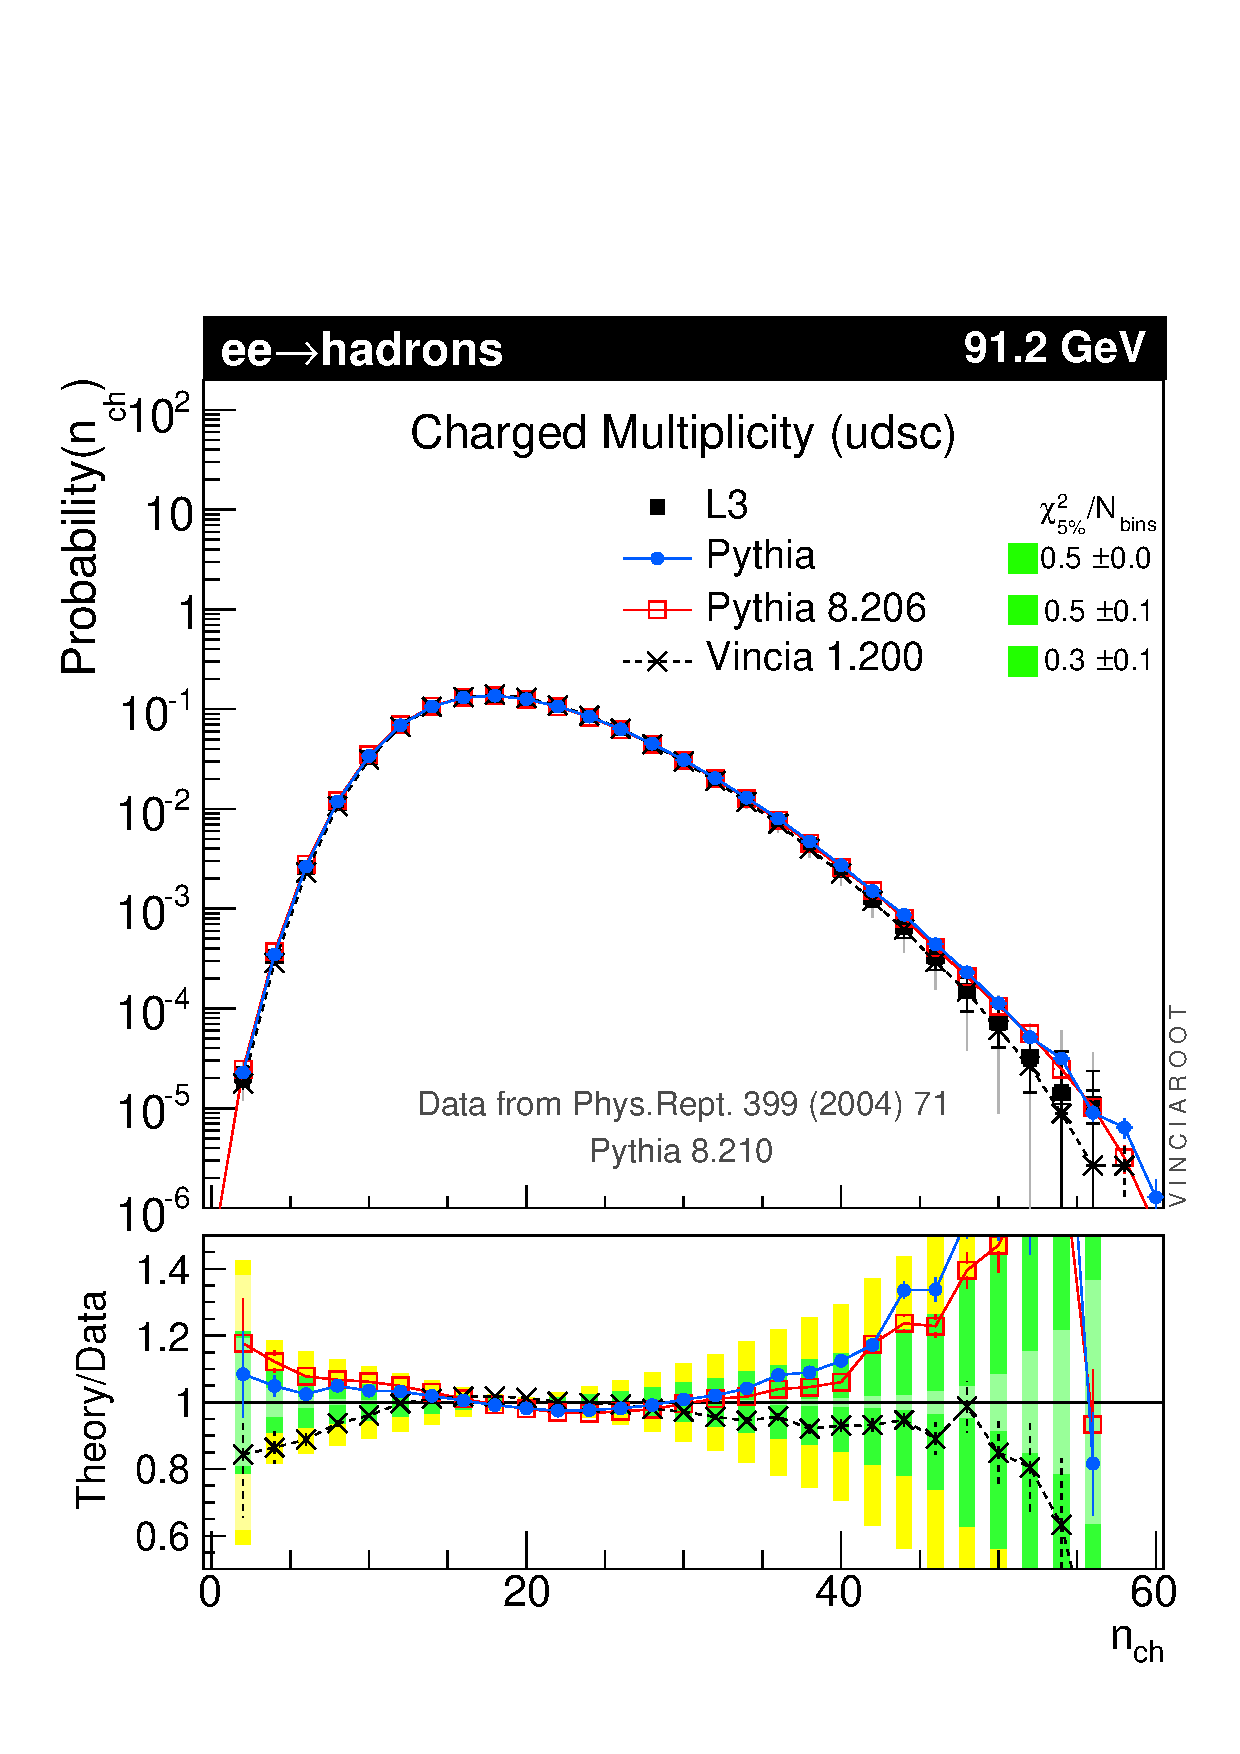
\includegraphics[width=5cm, height=5cm]{Vincia-T1/vincia03-Nch.pdf}
 \caption{$\chi^2$ values computed for $x$- (left), $|\log(x_p)|$ (middle) and charged multiplicity (right) using
 \texttt{Vincia}. Input parameters are from the \texttt{T1} fit results.}
 \label{Chi2-1}
 \end{figure}
 
  \begin{figure}[!h]
 \centering
 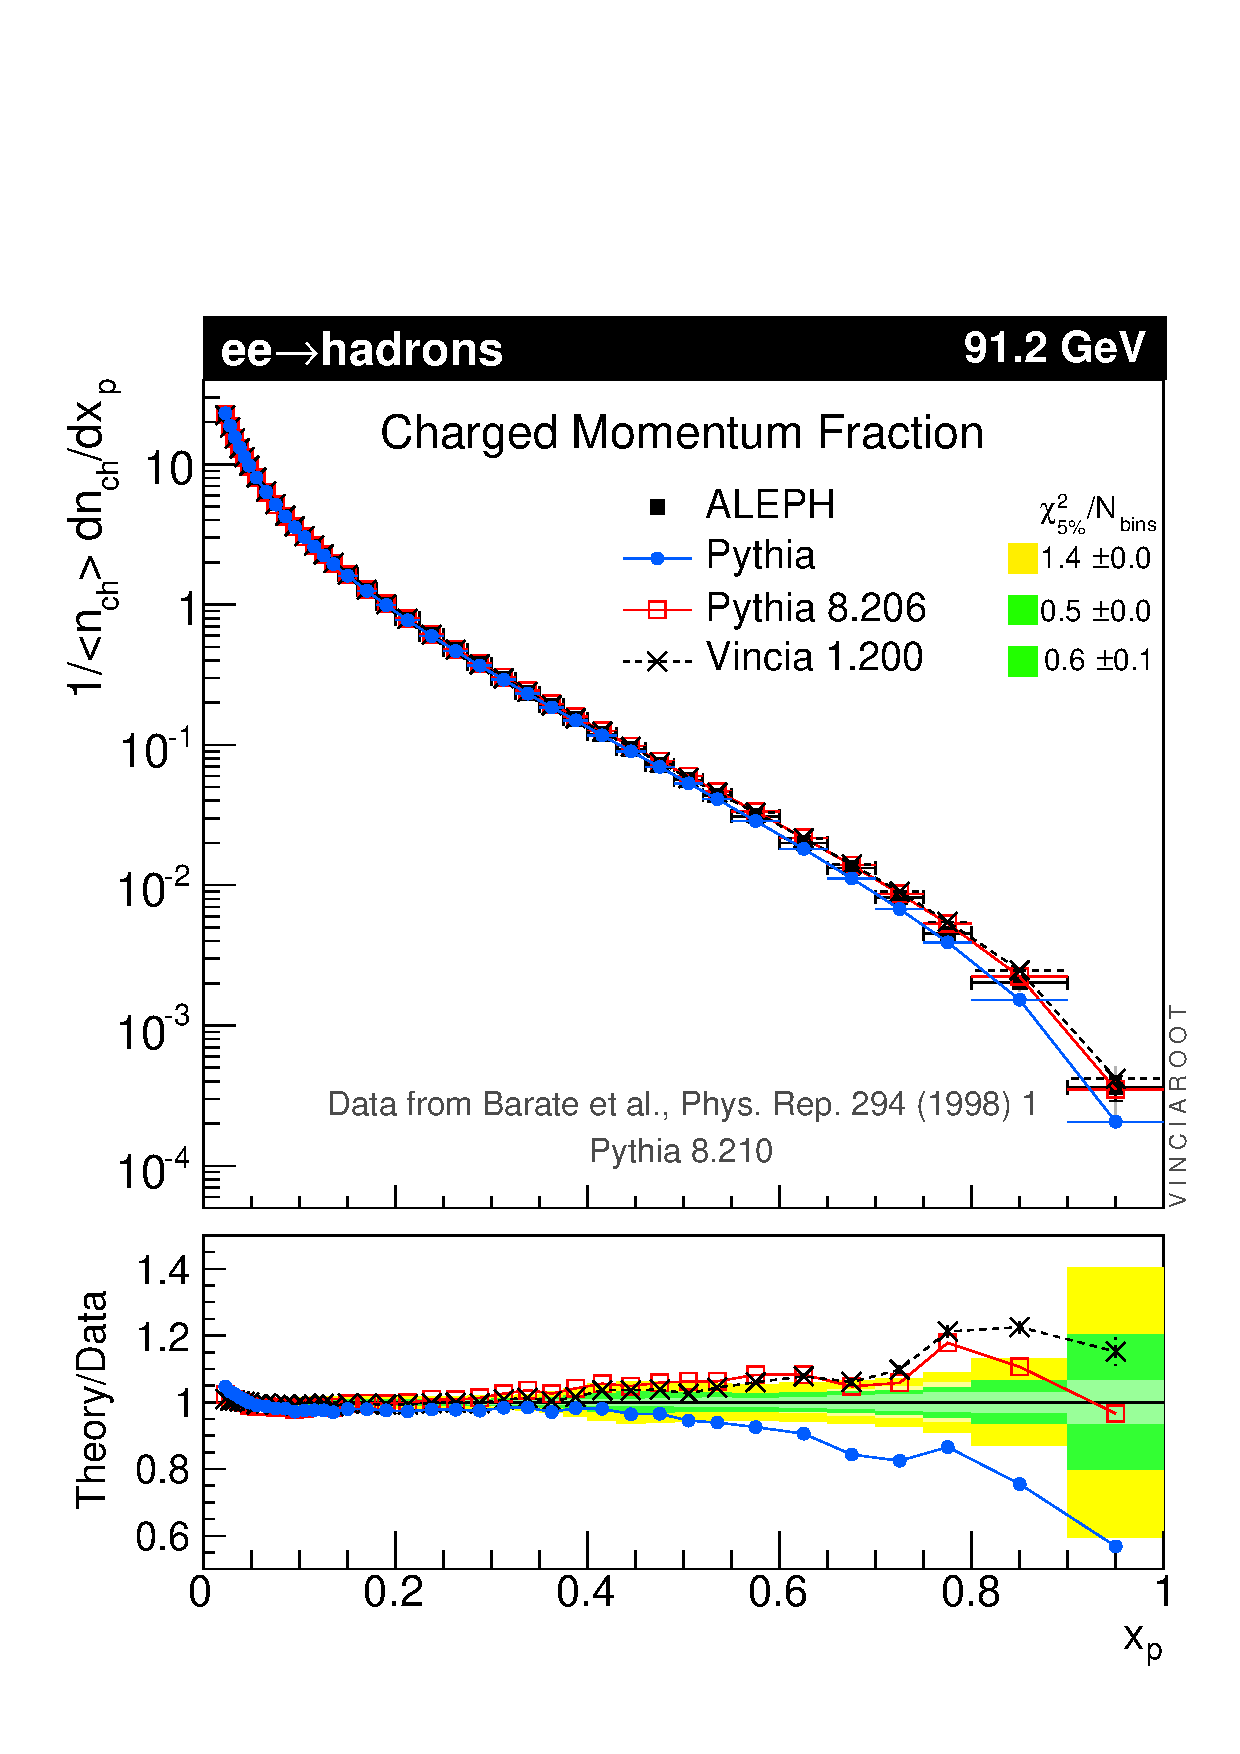
\includegraphics[width=5cm, height=5cm]{Vincia-T2/vincia03-x.pdf}
 \hfill
 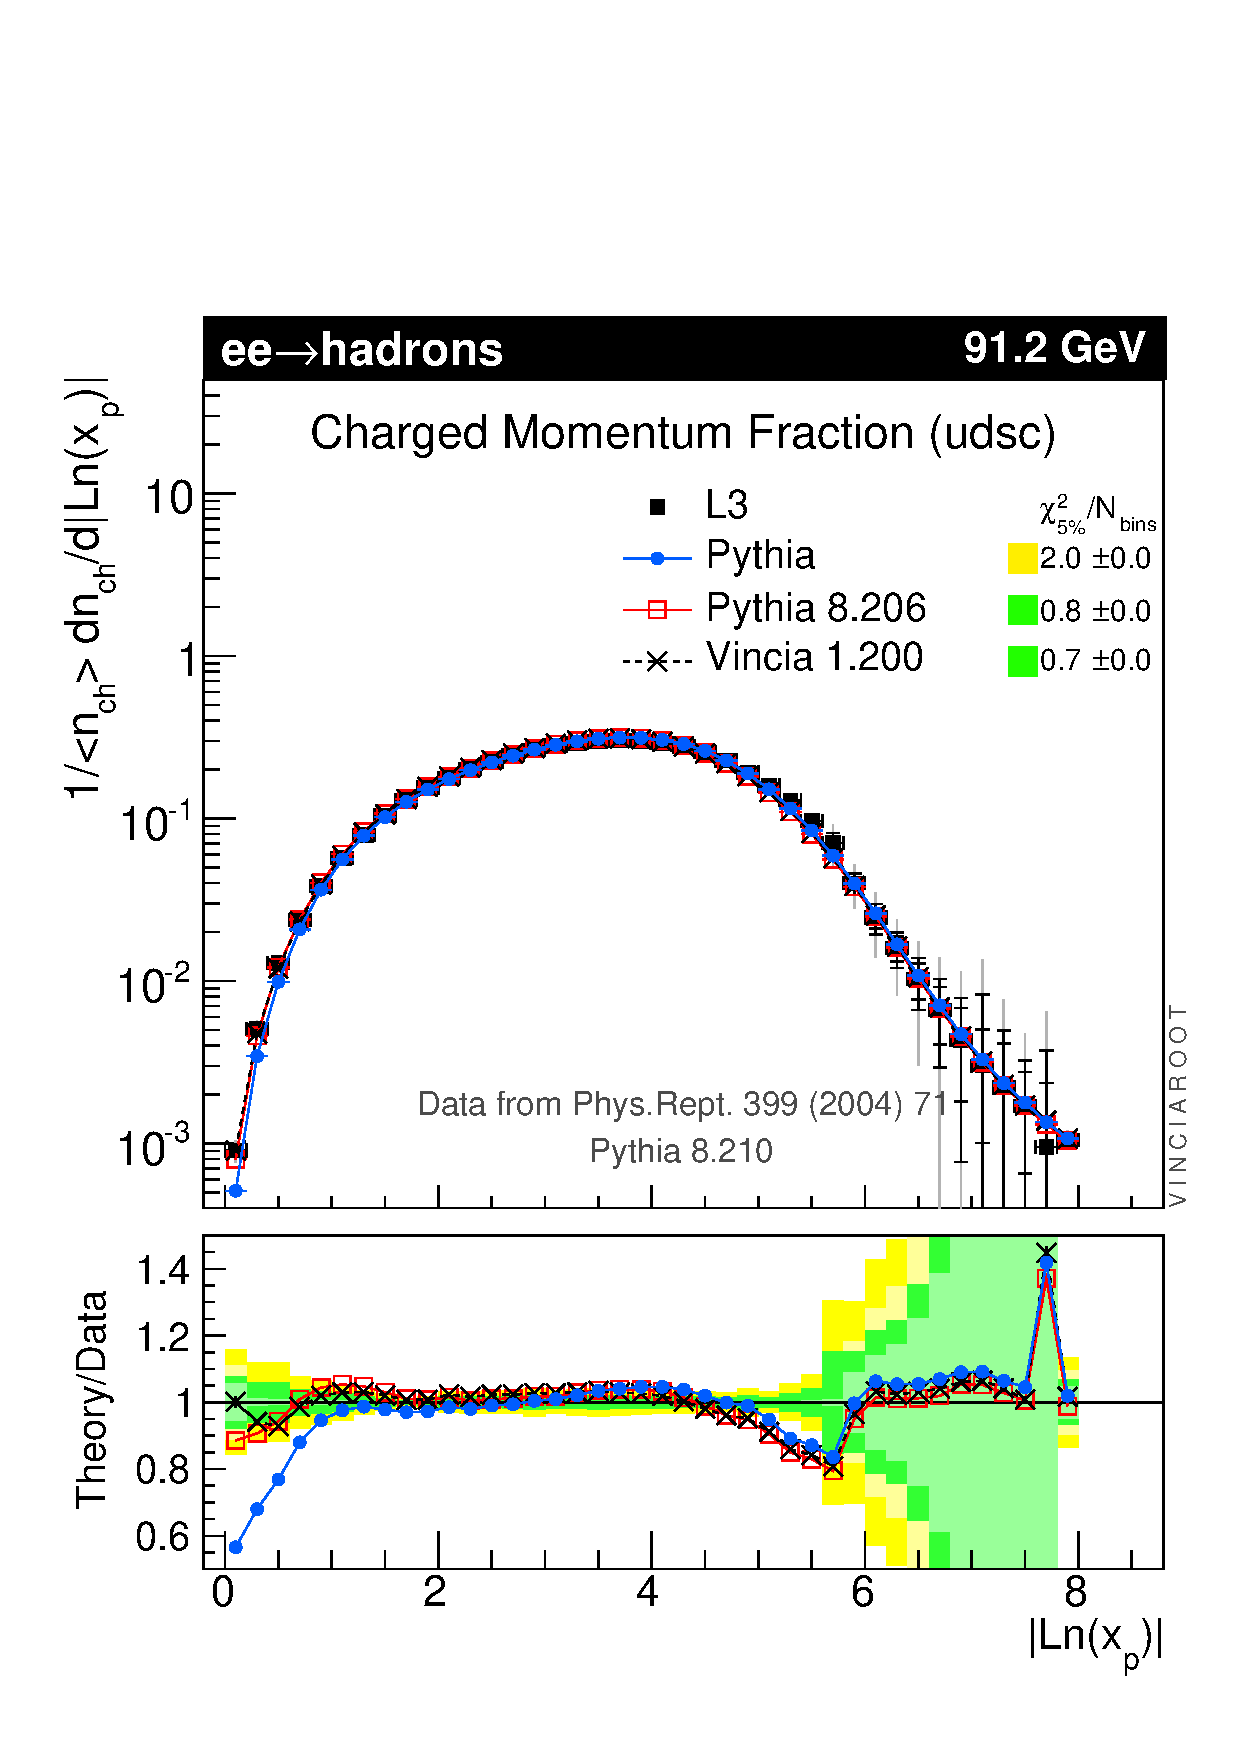
\includegraphics[width=5cm, height=5cm]{Vincia-T2/vincia03-Lnx.pdf}
 \hfill
 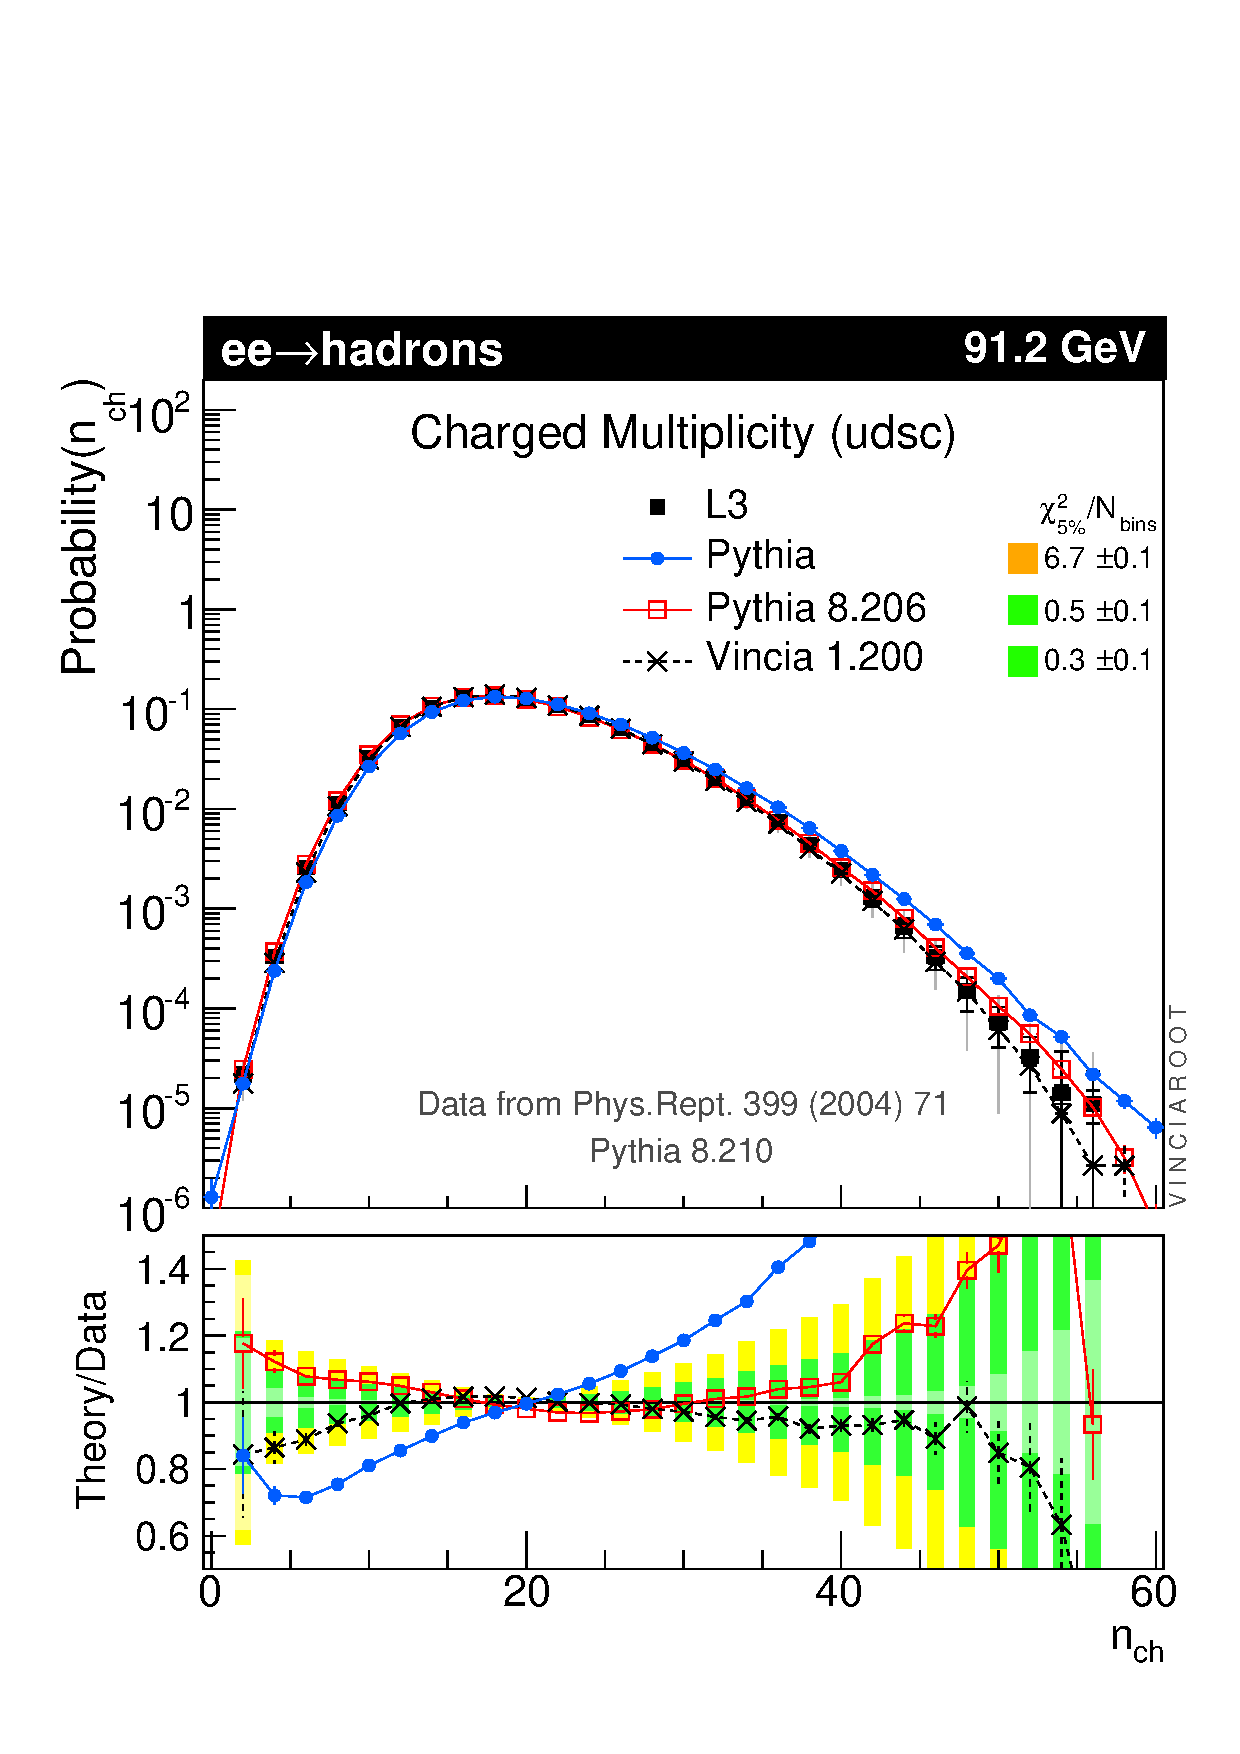
\includegraphics[width=5cm, height=5cm]{Vincia-T2/vincia03-Nch.pdf}
 \caption{$\chi^2$ values computed for $x$- (left), $|\log(x_p)|$ (middle) and charged multiplicity (right) using
 \texttt{Vincia}. Input parameters are from the \texttt{T2} fit results.}
 \label{Chi2-2}
 \end{figure}
 
   \begin{figure}[!h]
 \centering
 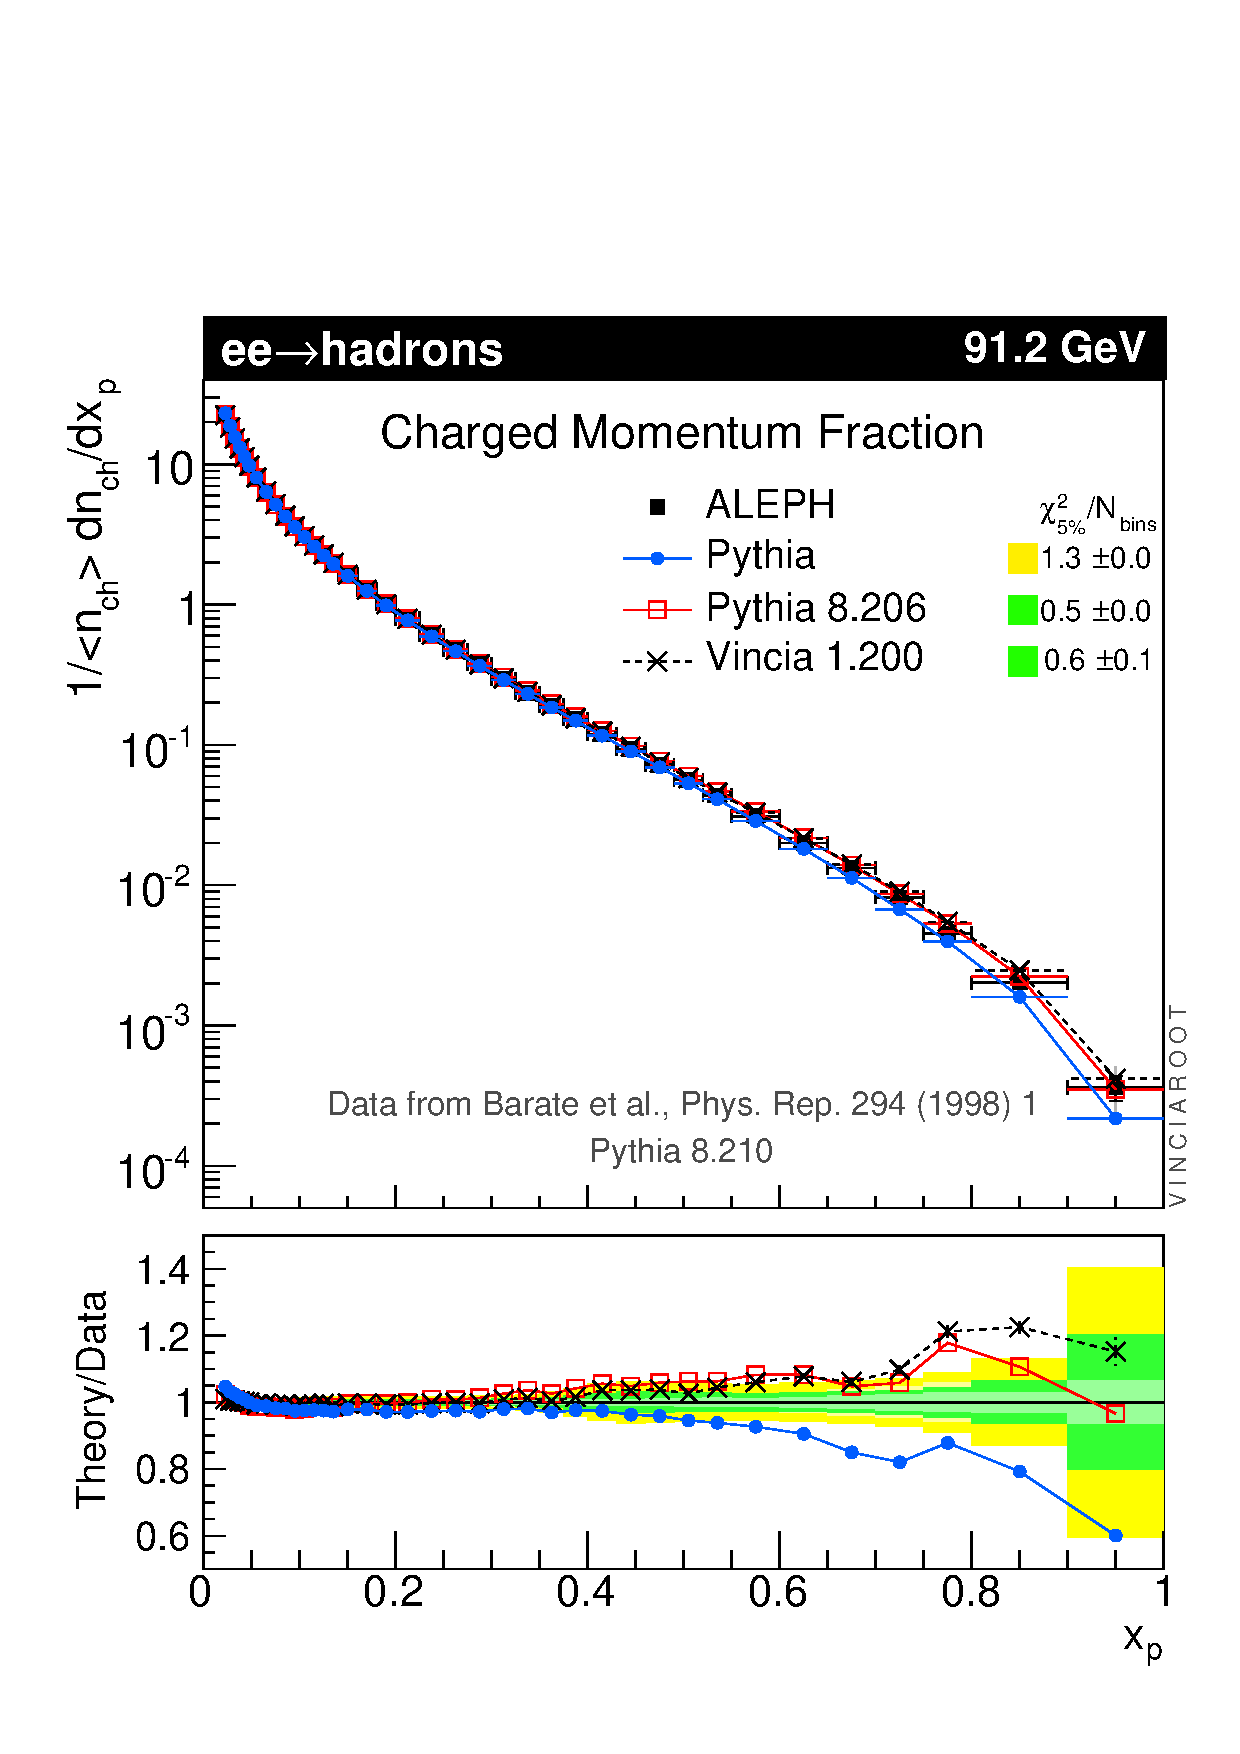
\includegraphics[width=5cm, height=5cm]{Vincia-T3/vincia03-x.pdf}
 \hfill
 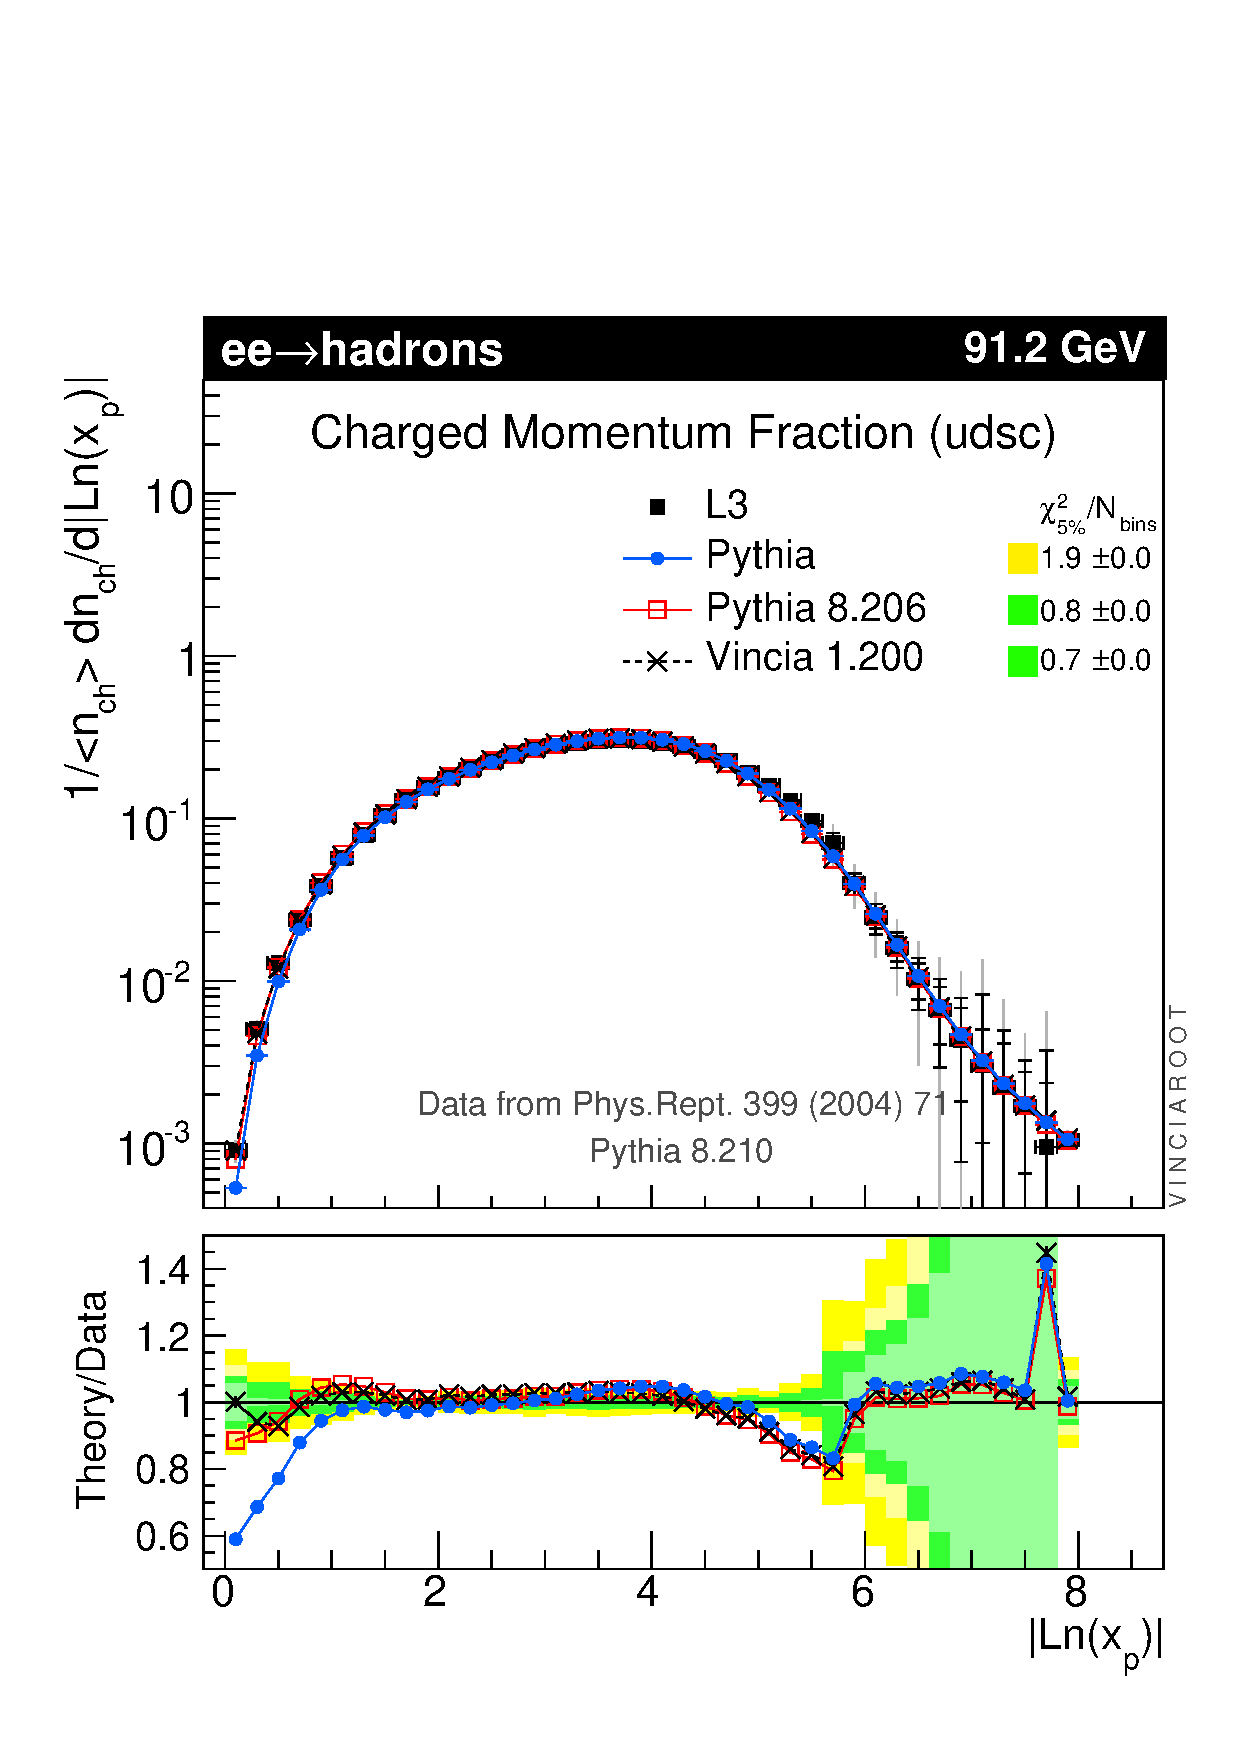
\includegraphics[width=5cm, height=5cm]{Vincia-T3/vincia03-Lnx.pdf}
 \hfill
 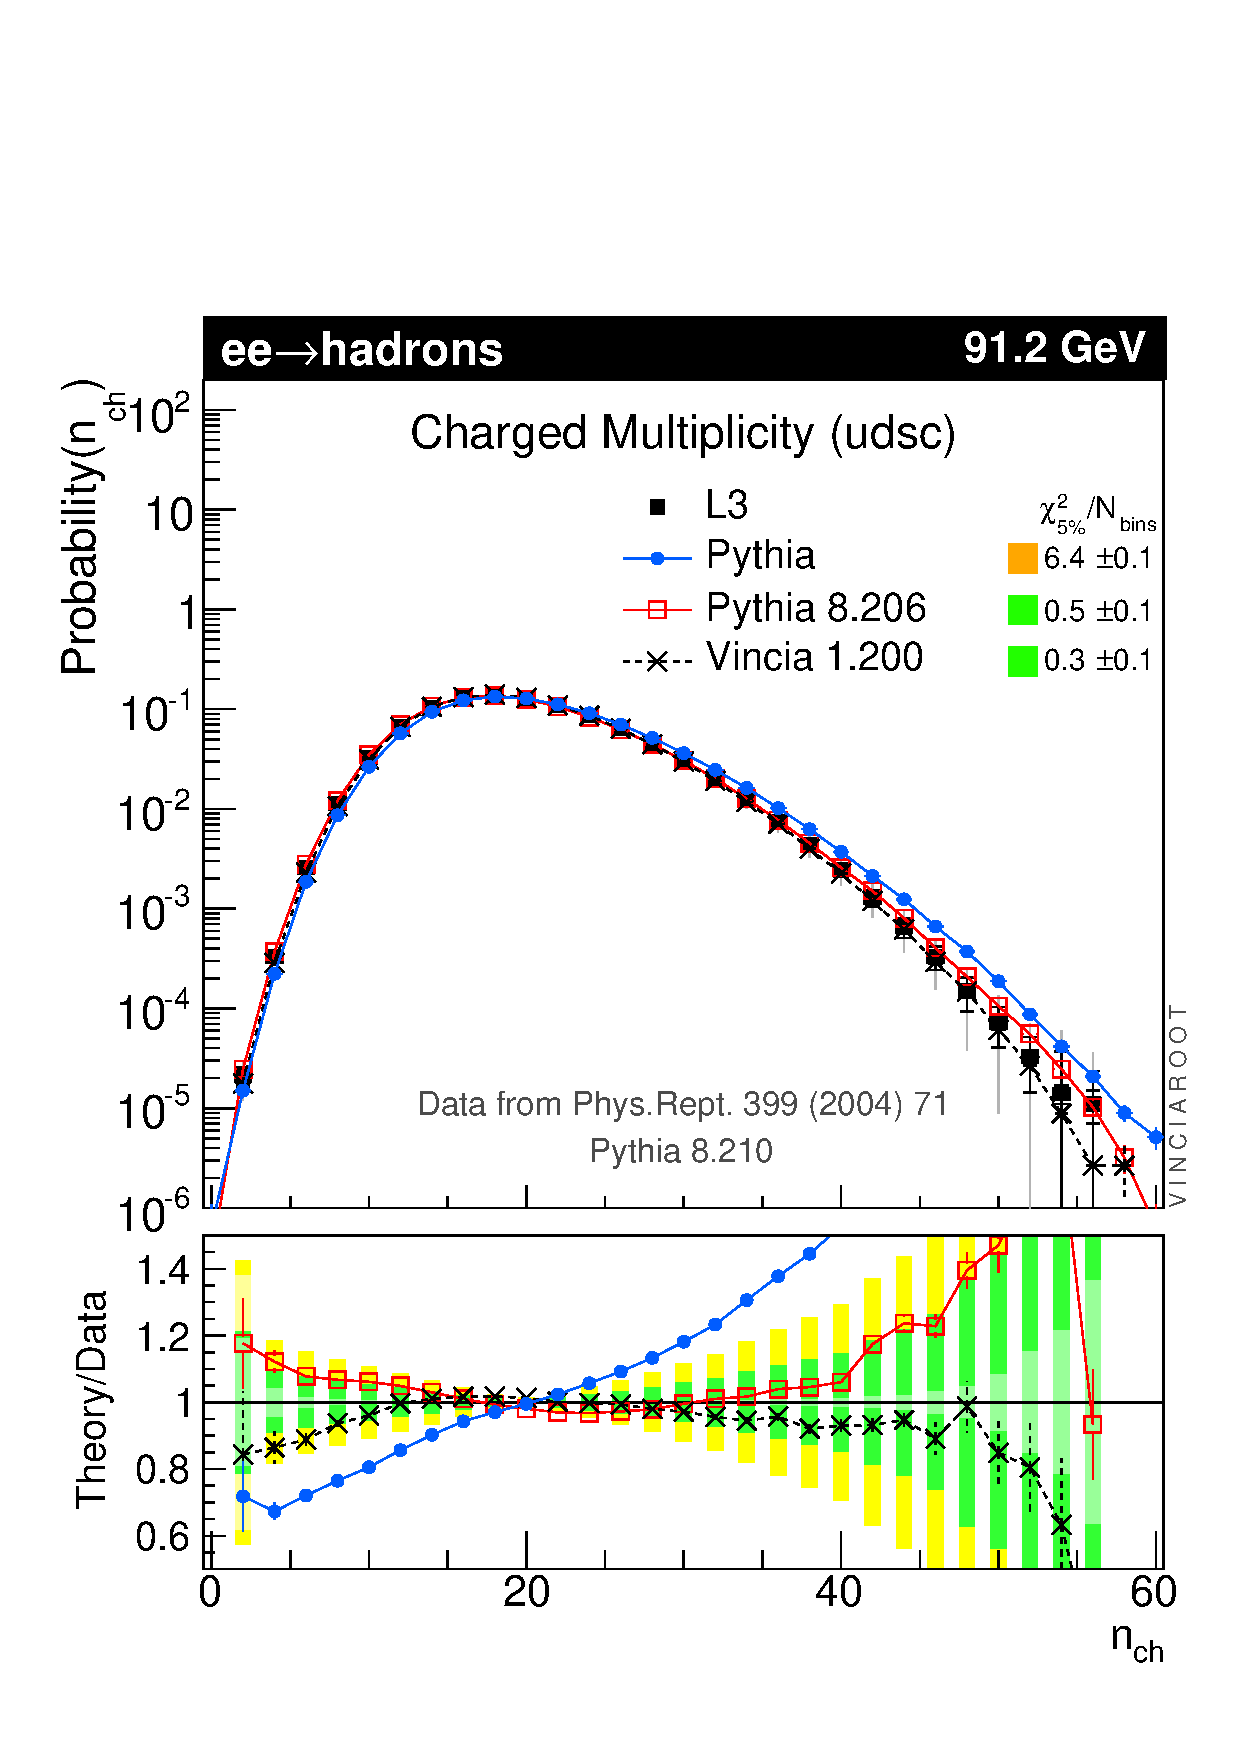
\includegraphics[width=5cm, height=5cm]{Vincia-T3/vincia03-Nch.pdf}
 \caption{$\chi^2$ values computed for $x$- (left), $|\log(x_p)|$ (middle) and charged multiplicity (right) using
 \texttt{Vincia}. Input parameters are from the \texttt{T3} fit results.}
 \label{Chi2-3}
 \end{figure}
 
   \begin{figure}[!h]
 \centering
 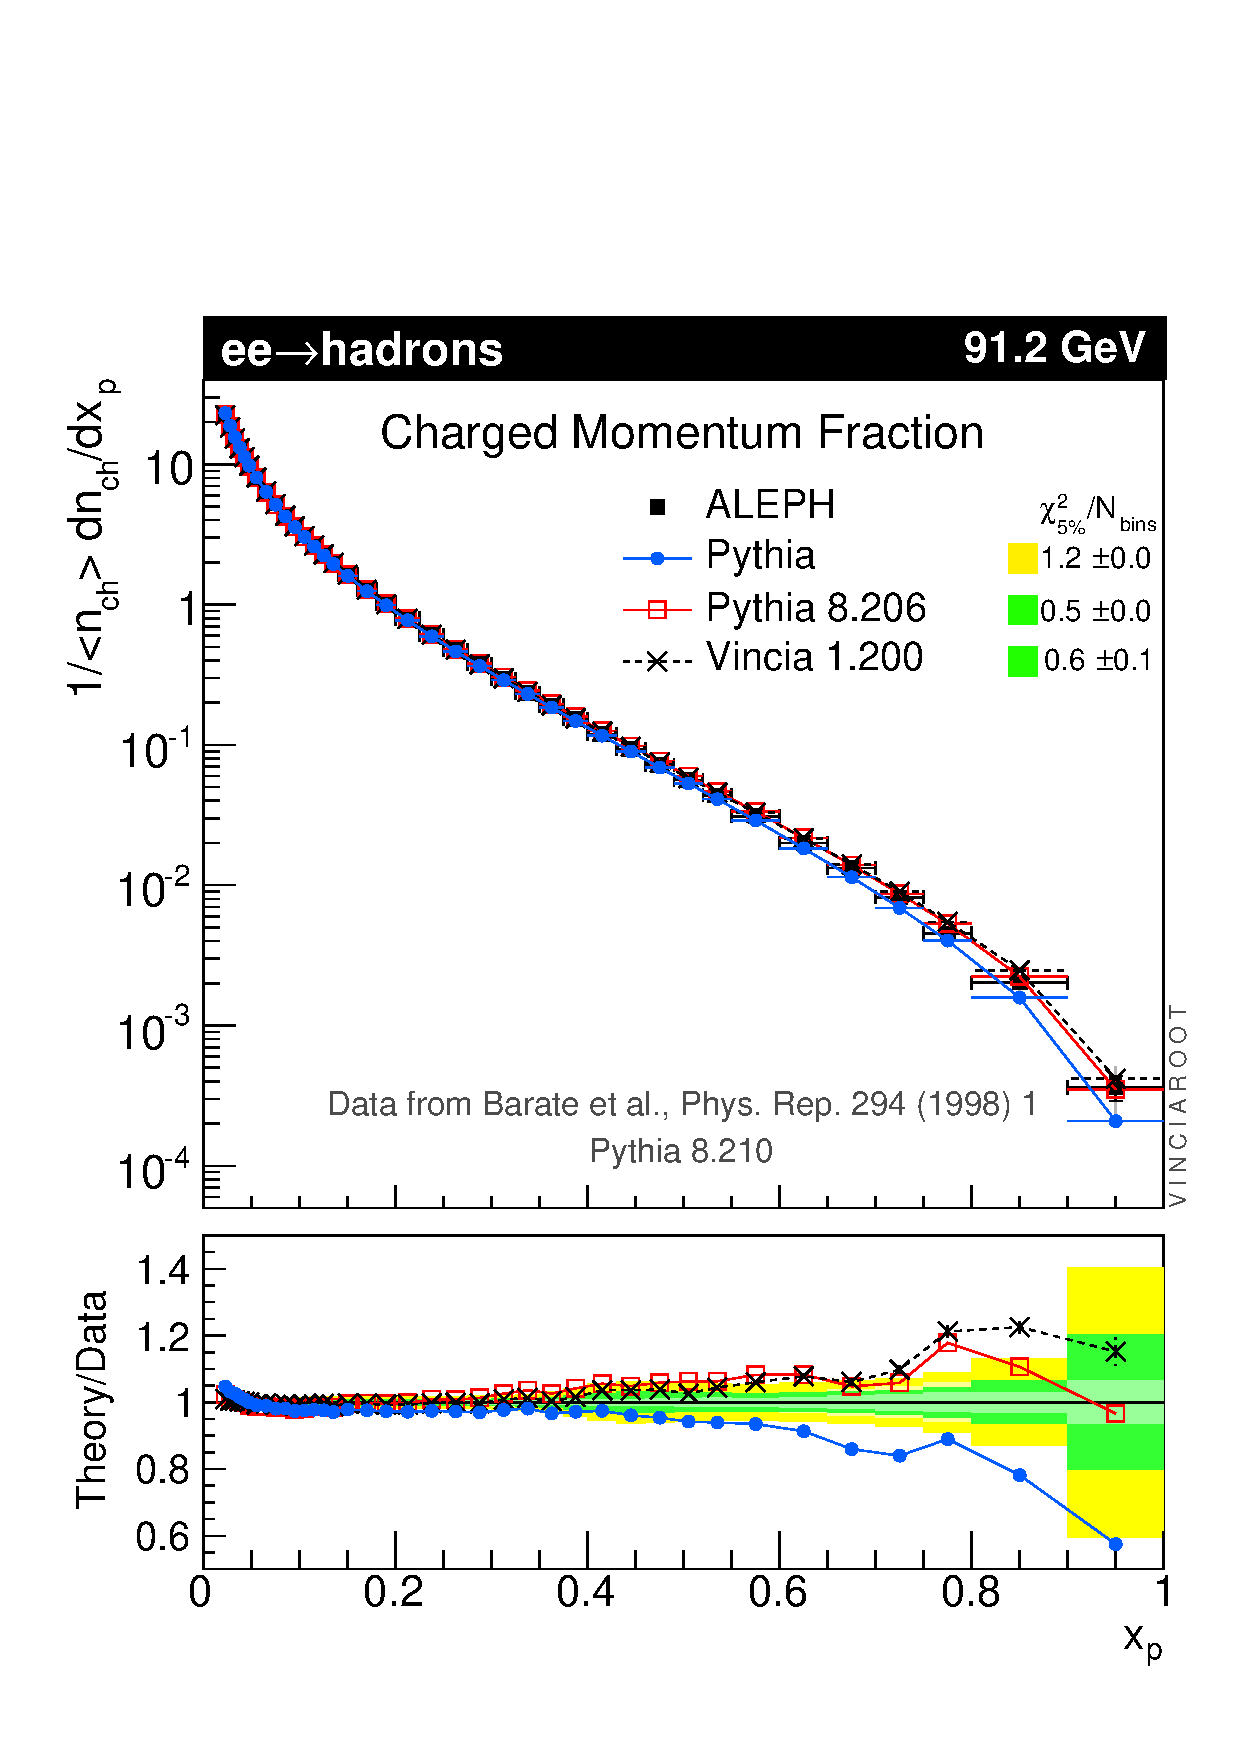
\includegraphics[width=5cm, height=5cm]{Vincia-T4/vincia03-x.pdf}
 \hfill
 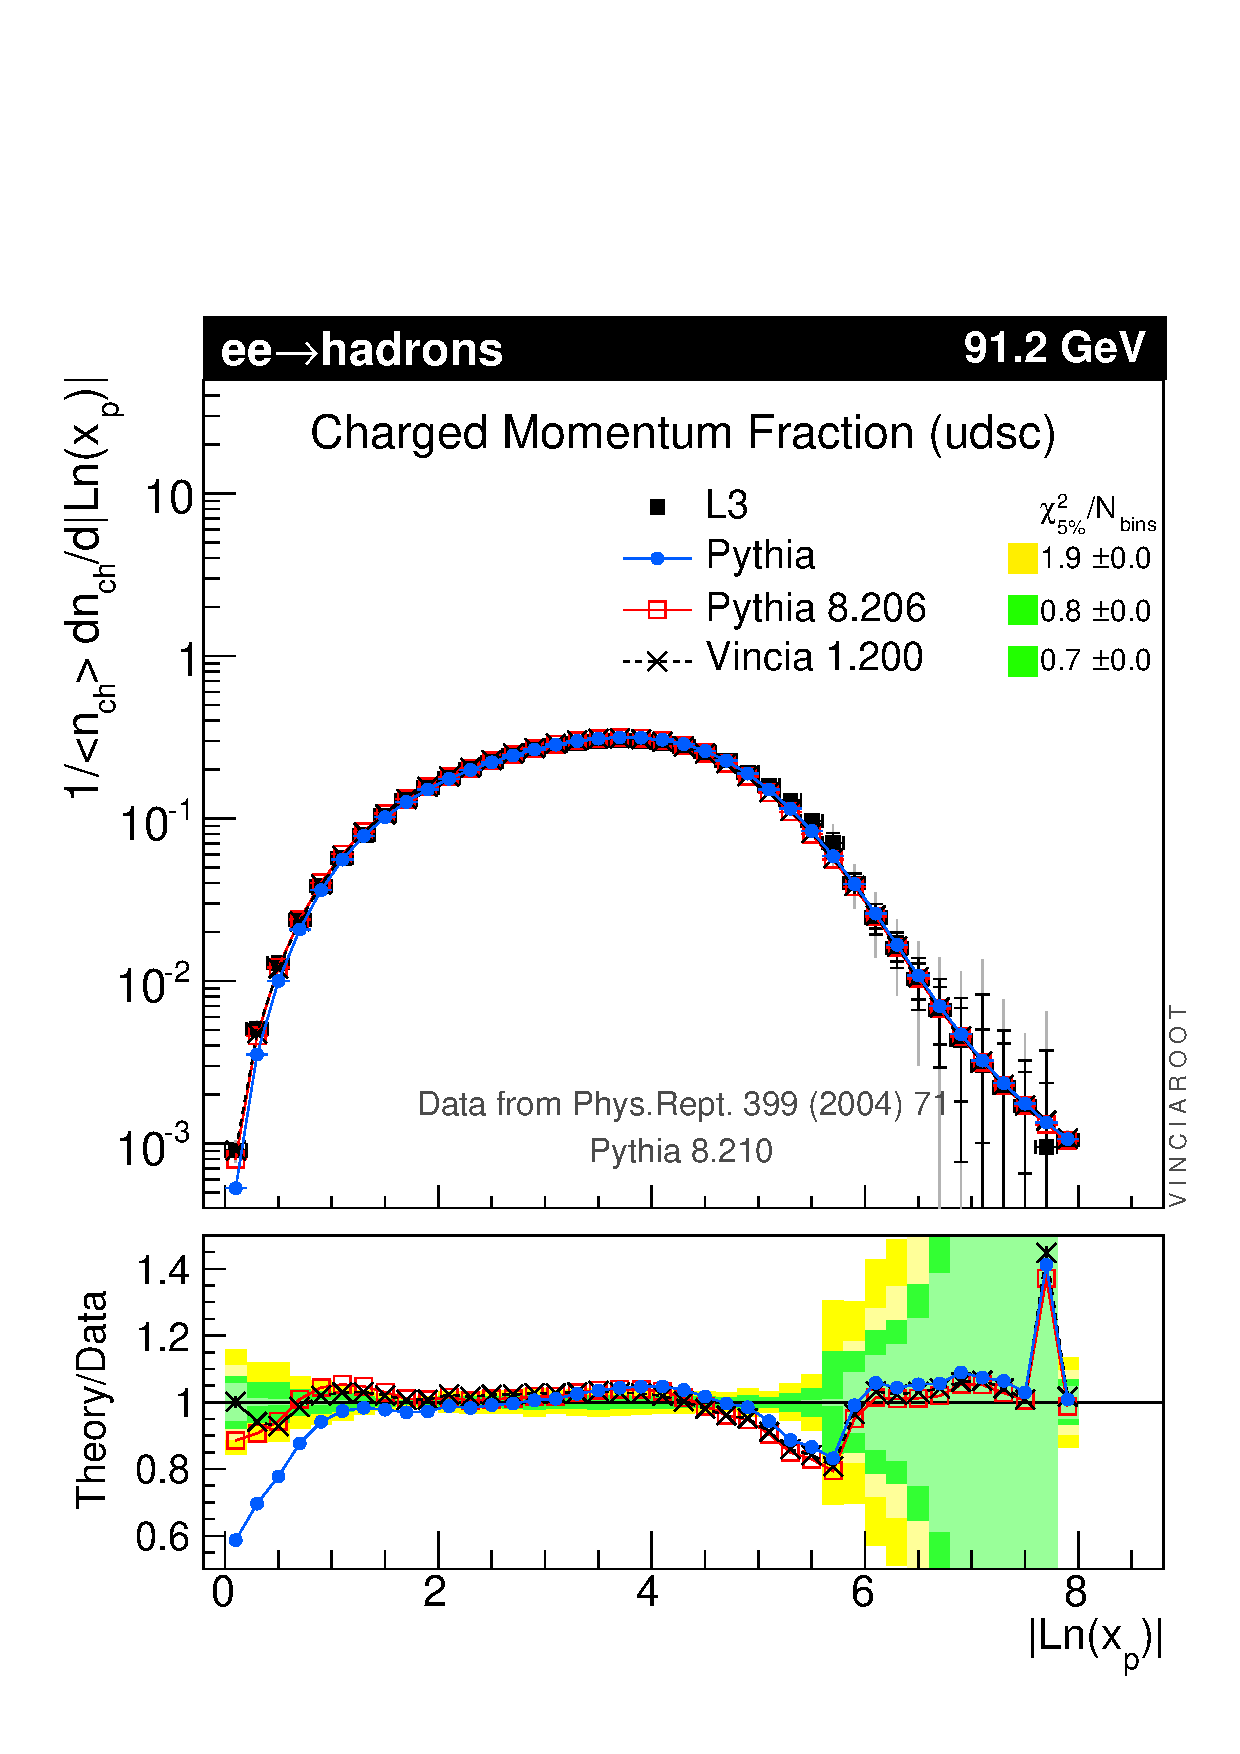
\includegraphics[width=5cm, height=5cm]{Vincia-T4/vincia03-Lnx.pdf}
 \hfill
 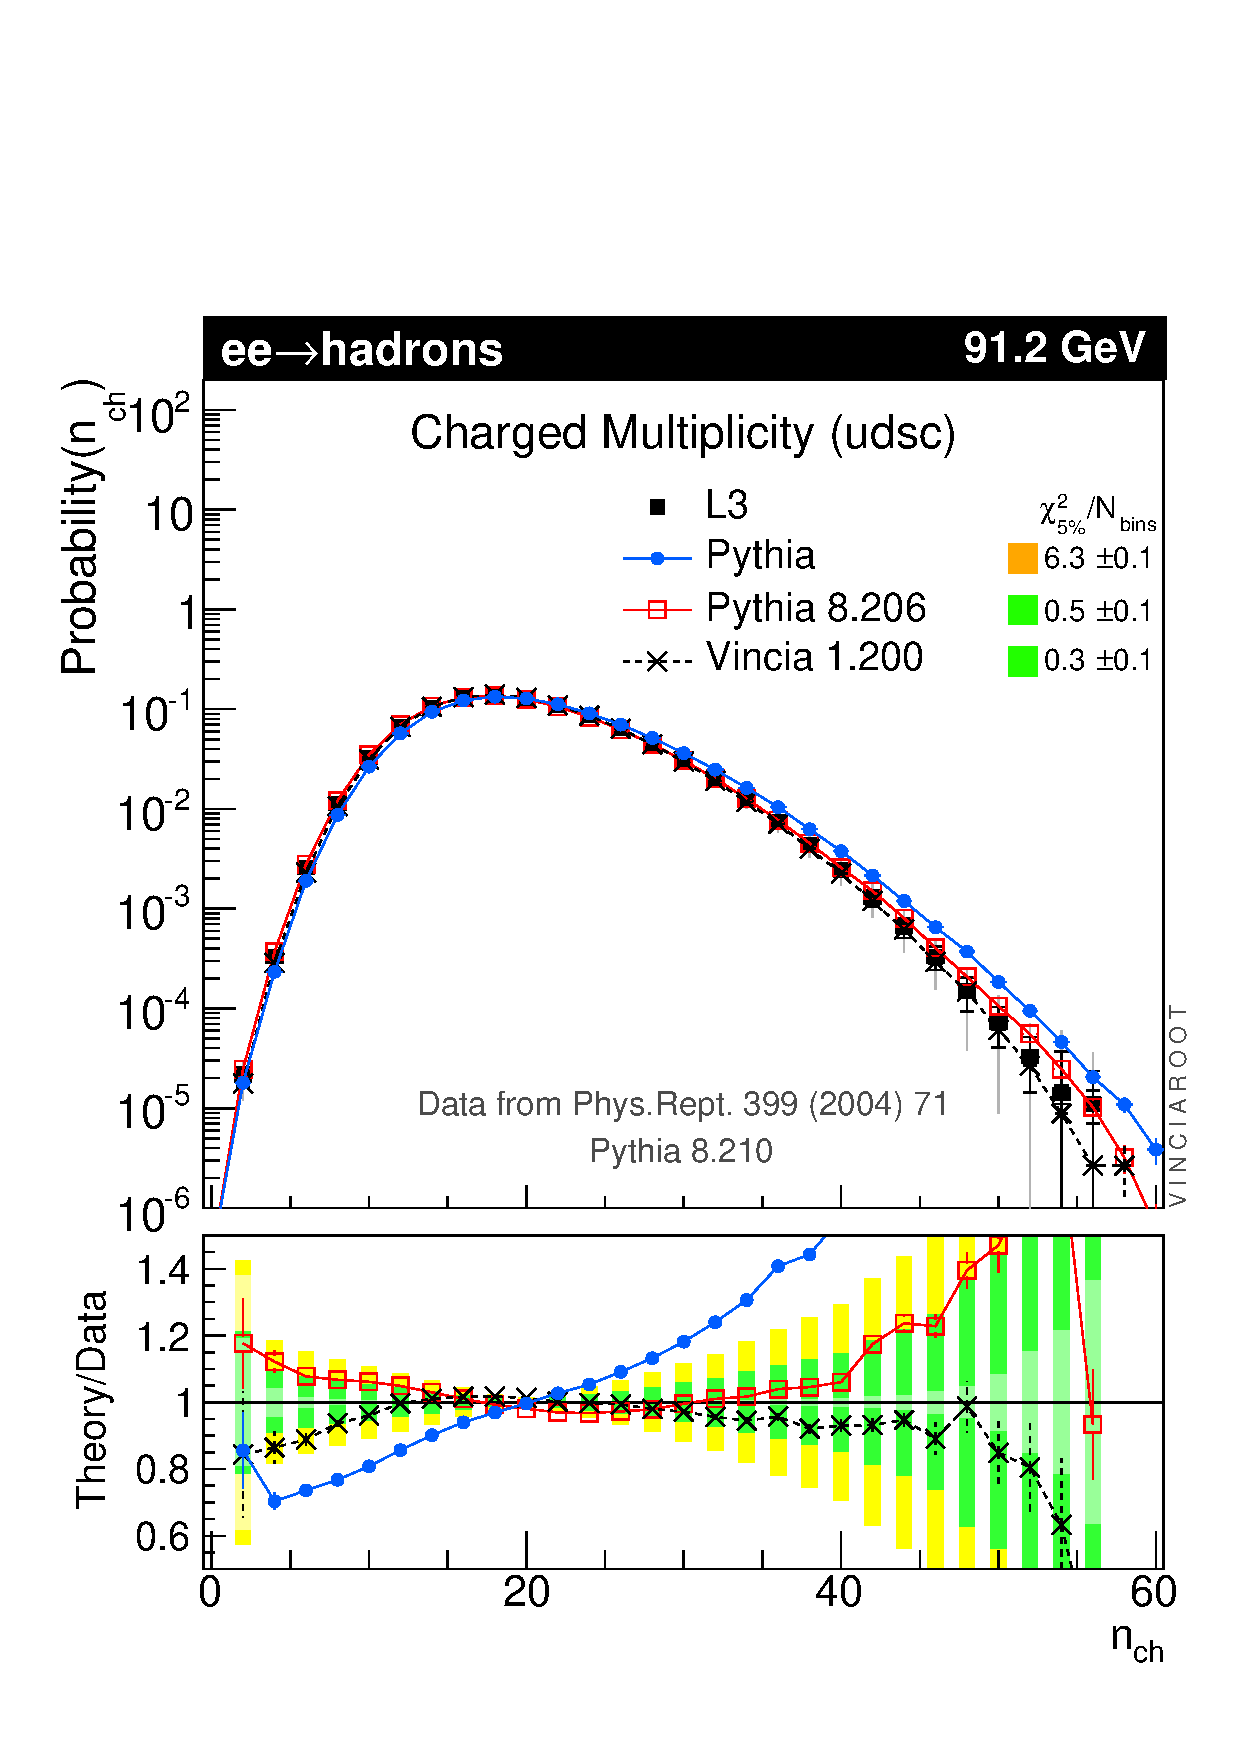
\includegraphics[width=5cm, height=5cm]{Vincia-T4/vincia03-Nch.pdf}
 \caption{$\chi^2$ values computed for $x$- (left), $|\log(x_p)|$ (middle) and charged multiplicity (right) using
 \texttt{Vincia}. Input parameters are from the \texttt{T3} fit results.}
 \label{Chi2-4}
 \end{figure}
 
   \begin{figure}[!h]
 \centering
 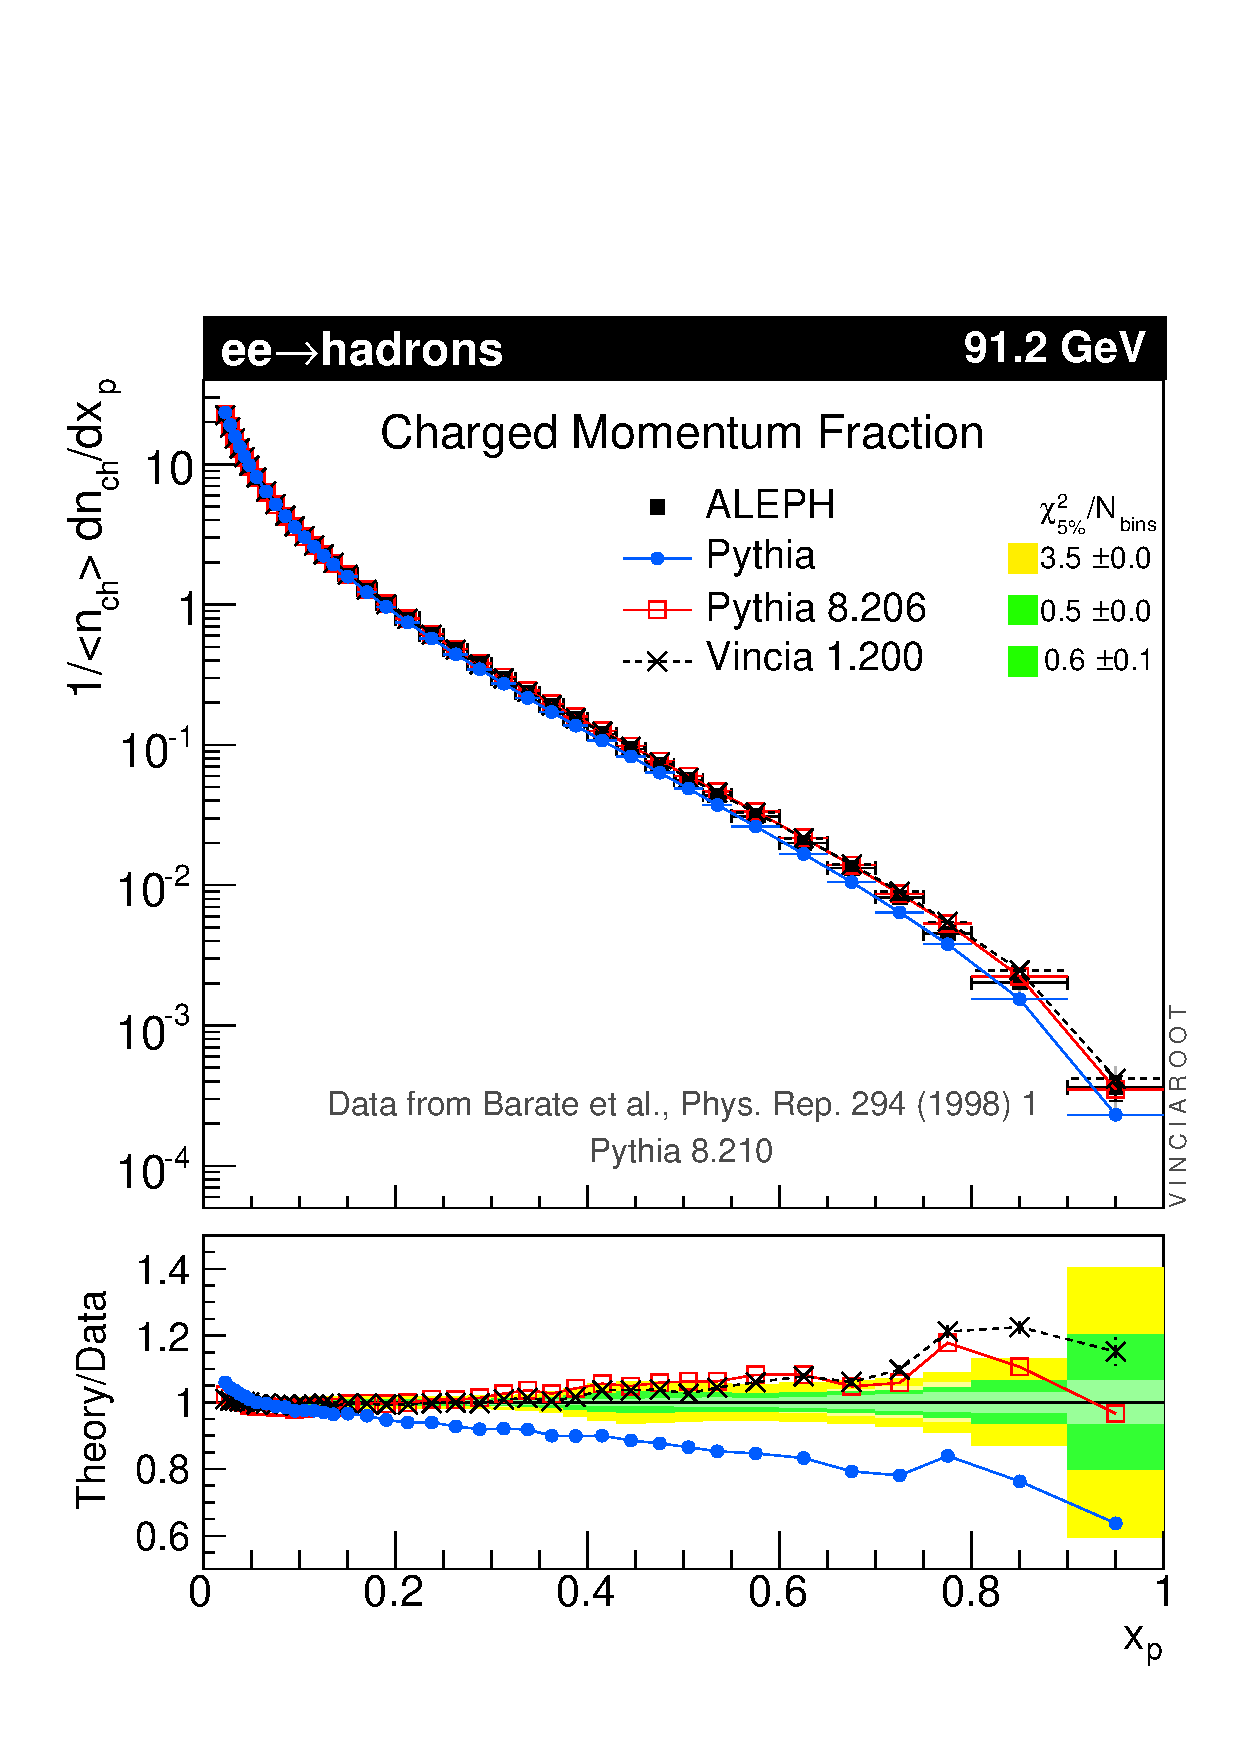
\includegraphics[width=5cm, height=5cm]{Vincia-T5/vincia03-x.pdf}
 \hfill
 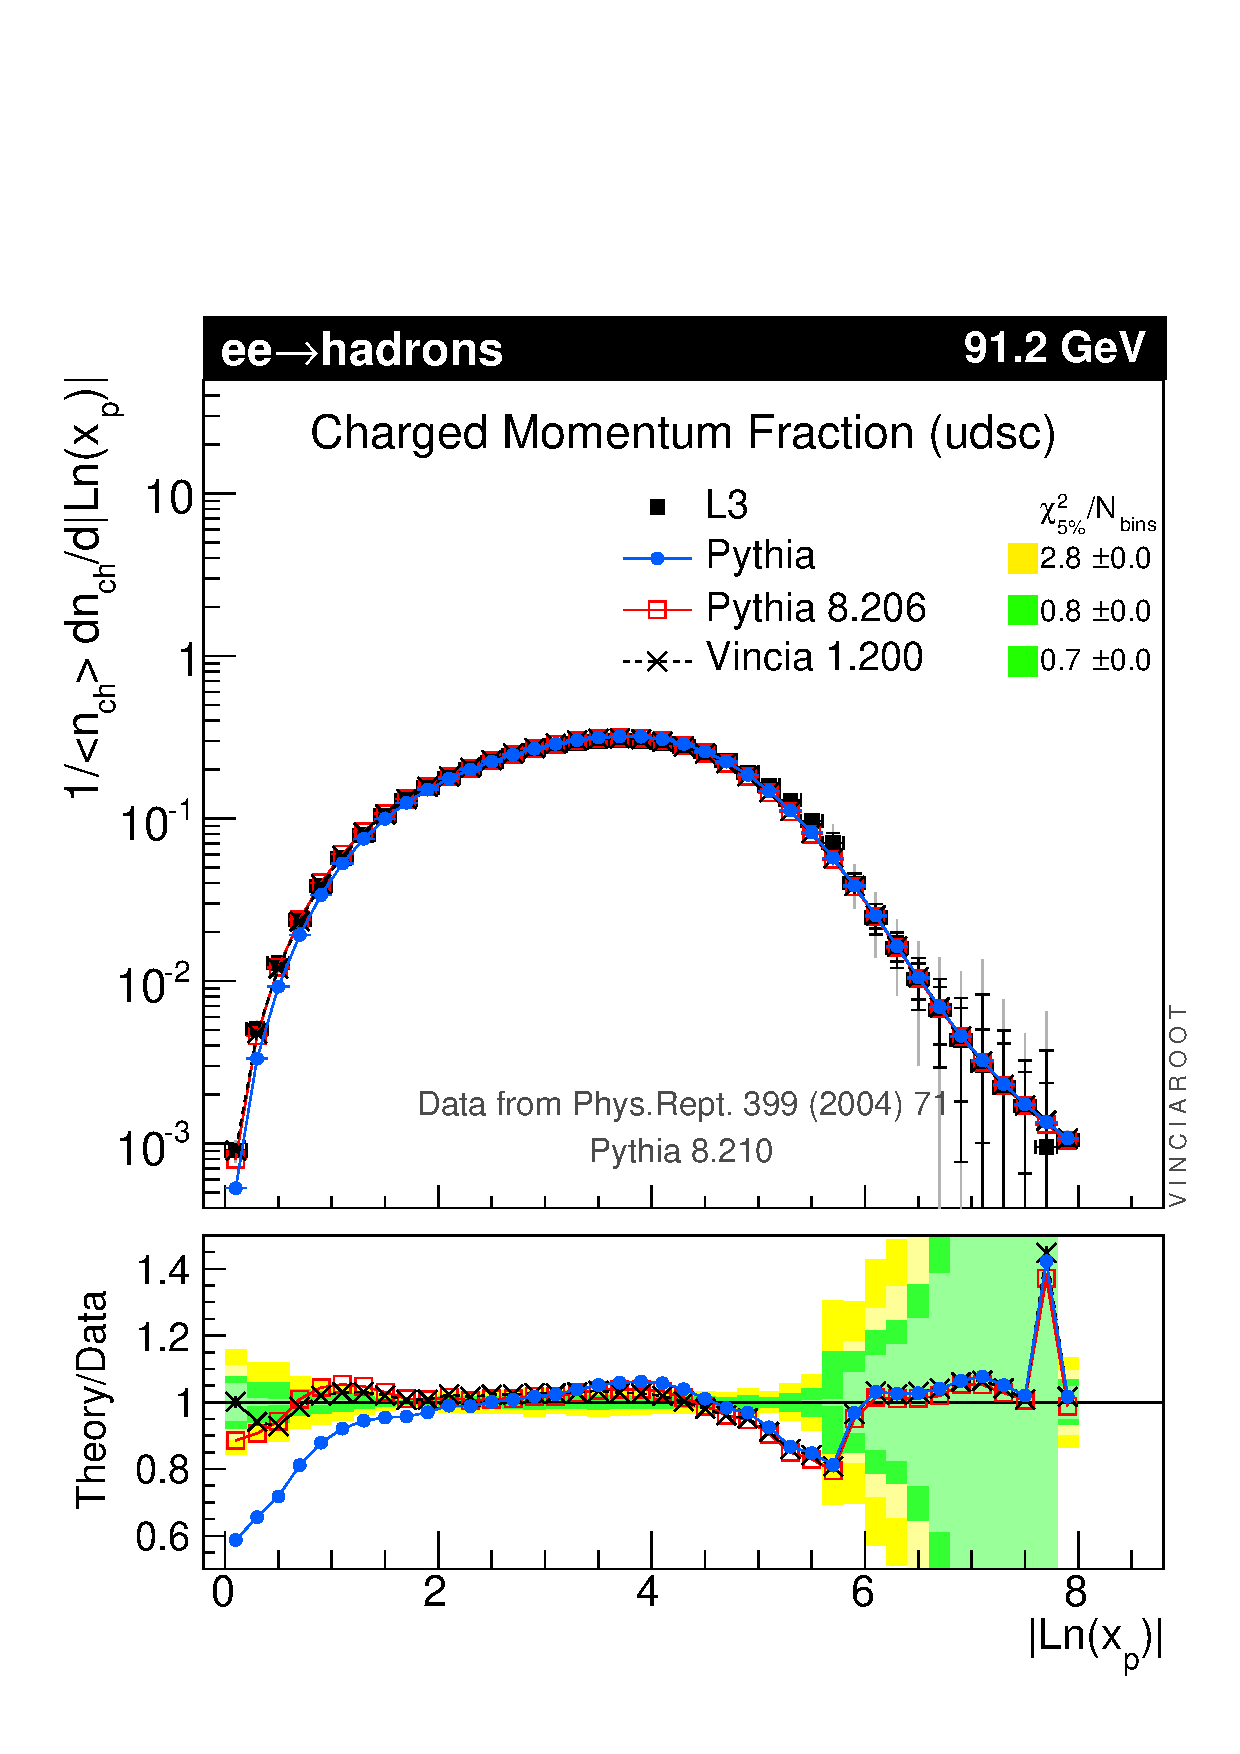
\includegraphics[width=5cm, height=5cm]{Vincia-T5/vincia03-Lnx.pdf}
 \hfill
 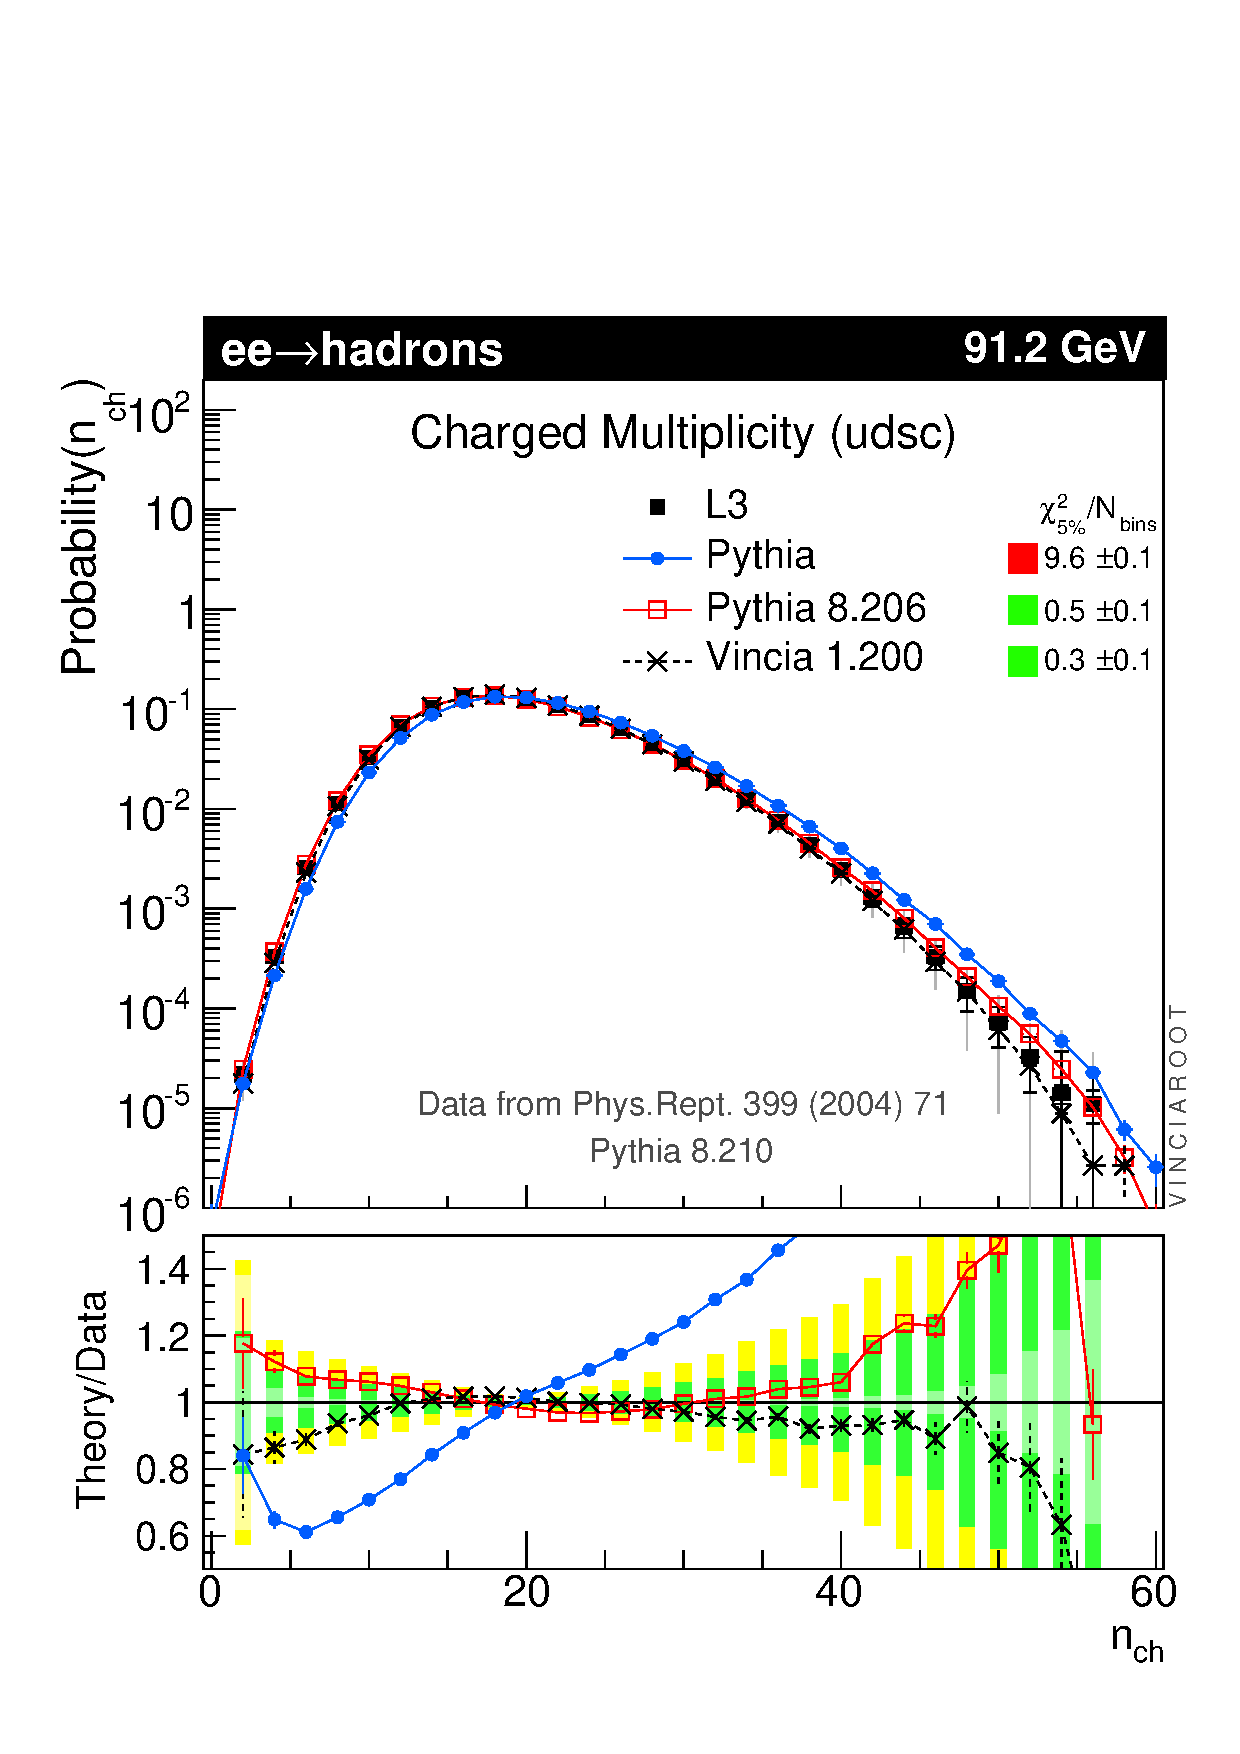
\includegraphics[width=5cm, height=5cm]{Vincia-T5/vincia03-Nch.pdf}
 \caption{$\chi^2$ values computed for $x$- (left), $|\log(x_p)|$ (middle) and charged multiplicity (right) using
 \texttt{Vincia}. Input parameters are from the \texttt{T5} fit results.}
 \label{Chi2-5}
 \end{figure}

 \begin{table}[tbp]
  \begin{center}
   \begin{tabular}{l|l|l|l|l}
    \hline \hline
    Parameter \hspace{1cm} & \hspace{1cm} $\Delta\sigma(\texttt{T1}) = +1 $ & \hspace{1cm} $\Delta\sigma(\texttt{T1}) = -1 $ & \hspace{1cm} $\Delta\sigma(\texttt{T2}) = +1 $ & \hspace{1cm} $\Delta\sigma(\texttt{T2}) = -1 $\\ \hline
    $a_L$     \hspace{1cm} & \hspace{1cm} $0.88$      &  \hspace{1cm} $0.7$ & \hspace{1cm} $0.8073$  & \hspace{1cm}  $1.139$ \\ \hline
    $b_L$     \hspace{1cm} & \hspace{1cm} $1.1$      &  \hspace{1cm} $1.2$ & \hspace{1cm} $1.175$ & \hspace{1cm} $1.097$  \\ \hline 
    $p_\perp (\text{GeV})$ \hspace{1cm} & \hspace{1cm} $0.3$ &  \hspace{1cm} $0.3$ & \hspace{1cm} $0.3024$ &  \hspace{1cm} $0.3042$ \\ \hline
\hline
    \end{tabular}
  \end{center}
  \caption{Variation results of $a_L, b_L \text{ and } p_\perp$ using the manual method $\texttt{T1}$ and
  the \texttt{eigentune} method \texttt{T2}}
  \label{Variation-1}
 \end{table}
 
  \begin{table}[tbp]
  \begin{center}
   \begin{tabular}{l|l|l|l|l}
    \hline \hline
    Parameter \hspace{1cm} & \hspace{1cm} $\Delta\sigma(\texttt{T3}) = +1 $ & \hspace{1cm} $\Delta\sigma(\texttt{T3}) = -1 $ & \hspace{1cm} $\Delta\sigma(\texttt{T4}) = +1 $ & \hspace{1cm} $\Delta\sigma(\texttt{T4}) = -1 $\\ \hline
    $a_L$     \hspace{1cm} & \hspace{1cm} $0.9286$  &  \hspace{1cm} $0.9112$ & \hspace{1cm} $0.9181$  & \hspace{1cm}  $0.9004$ \\ \hline
    $b_L$     \hspace{1cm} & \hspace{1cm} $1.06$    &  \hspace{1cm} $1.06$ & \hspace{1cm} $1.048$ & \hspace{1cm} $1.048$  \\ \hline 
    $p_\perp (\text{GeV})$ \hspace{1cm} & \hspace{1cm} $0.277$ &  \hspace{1cm} $0.3431$ & \hspace{1cm} $0.2768$ &  \hspace{1cm} $0.3432$ \\ \hline
    \hline
    \end{tabular}
  \end{center}
  \caption{Variation results of $a_L, b_L \text{ and } p_\perp$ around the \texttt{T3} and \texttt{T4} fit results.}
  \label{Variation-2}
 \end{table}
 
 \begin{table}
  \begin{center}
   \begin{tabular}{l|l|l}
    \hline \hline
    Parameter \hspace{1cm} & \hspace{1cm} $\Delta\sigma(\texttt{T5}) = +1 $ & \hspace{1cm} $\Delta\sigma(\texttt{T5}) = -1 $ \\ \hline
    $a_L$     \hspace{1cm} & \hspace{1cm} $0.5676$       &  \hspace{1cm} $1.041$  \\ \hline
    $b_L$     \hspace{1cm} & \hspace{1cm} $0.5865$        &  \hspace{1cm} $0.7244$ \\ \hline
    $p_\perp (\text{GeV})$ \hspace{1cm} & \hspace{1cm} $0.3562$ &  \hspace{1cm} $0.346$ \\ \hline \hline
   \end{tabular}
  \end{center}
  \caption{Variation results of $a_L, b_L \text{ and } p_\perp$ around the \texttt{T5} fit results.}
  \label{Variation-3}
 \end{table}


 \begin{figure}[btp]
 \centering
 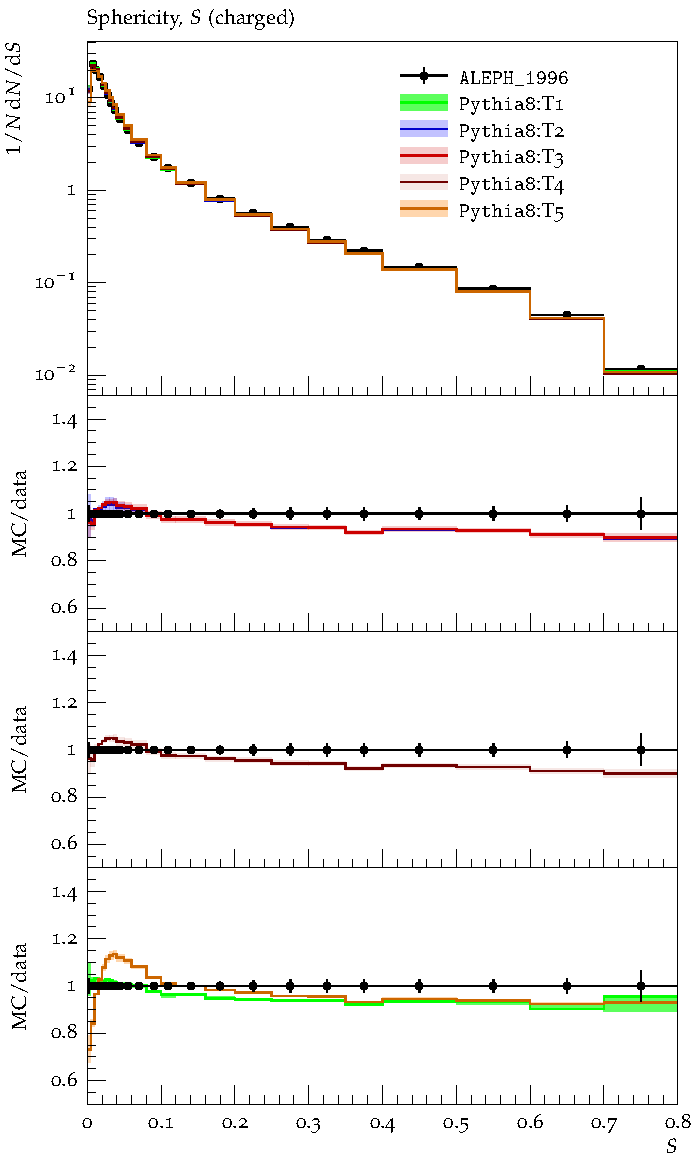
\includegraphics[width=8cm, height=9cm]{ALEPH_1996/d01-x01-y01.pdf}
 \hfill
  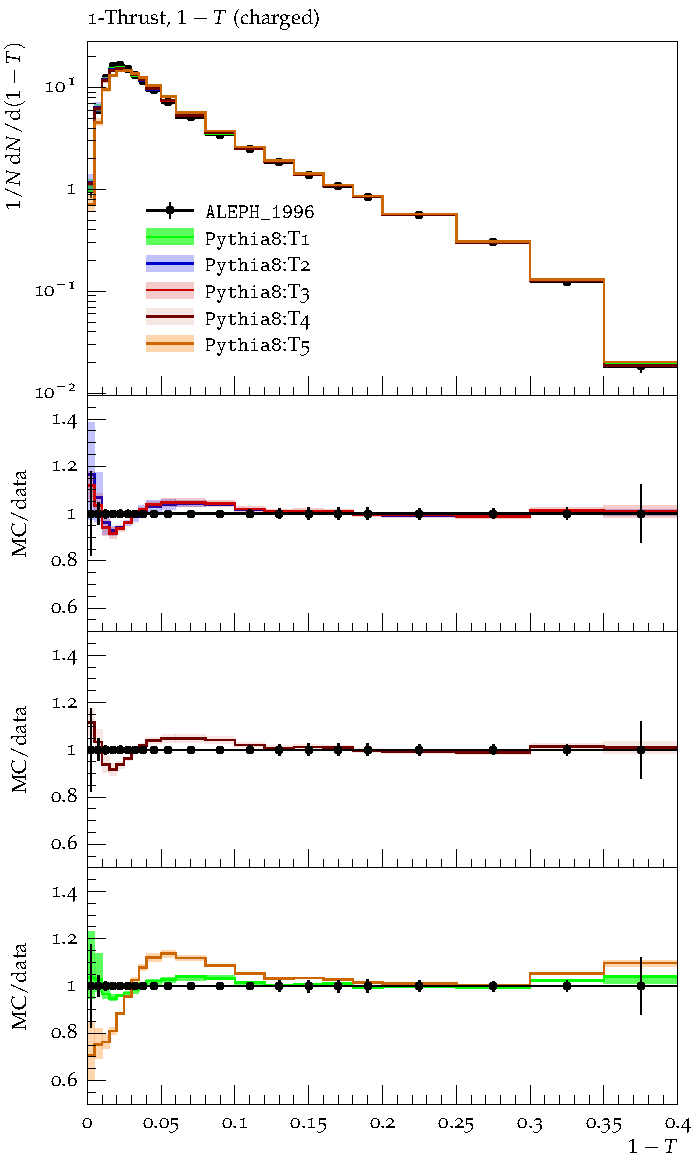
\includegraphics[width=8cm, height=9cm]{ALEPH_1996/d03-x01-y01.pdf}
  \caption{Sphericity (left) and Thrust (right) distributions. Data are taken from \cite{Barate:1996fi}.}
  \label{Fig-1}
 \end{figure} 
 

\begin{figure}[btp]
 \centering
 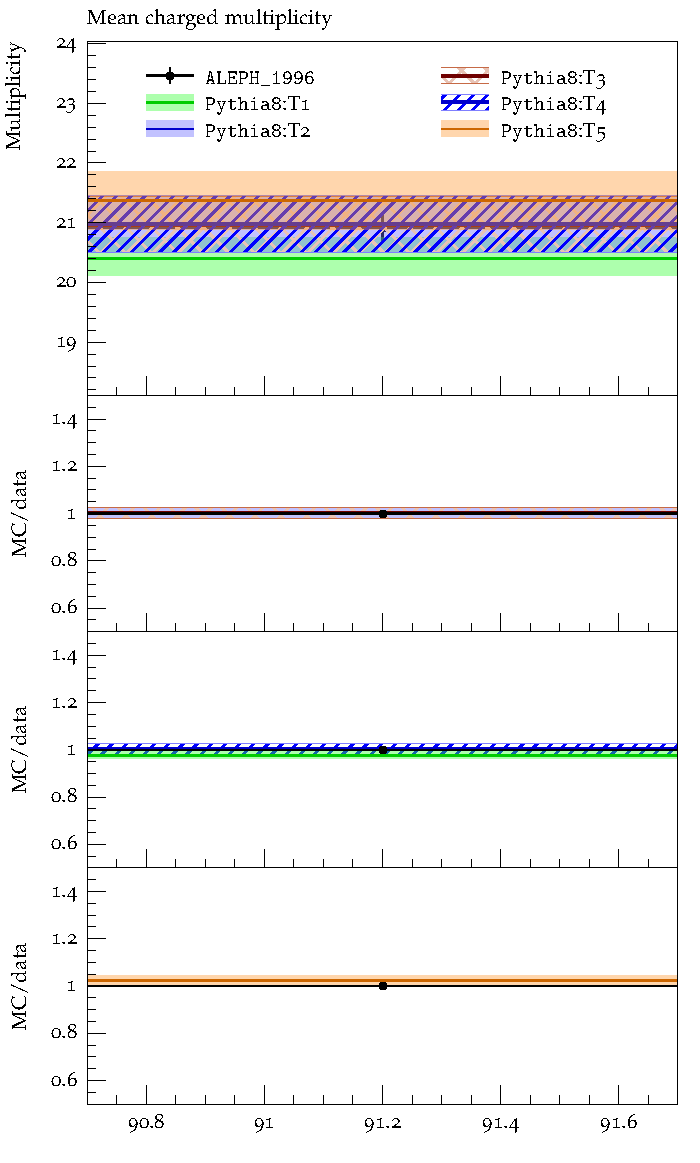
\includegraphics[width=8cm, height=9cm]{ALEPH_1996/d19-x01-y01.pdf}
 \hfill
  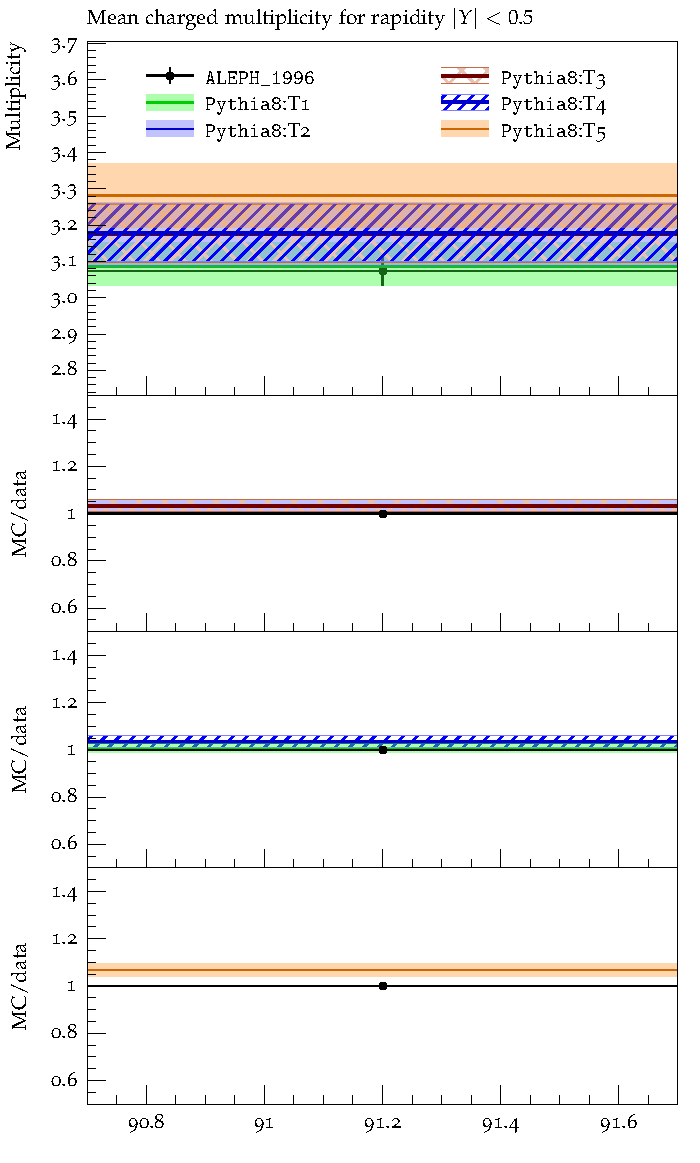
\includegraphics[width=8cm, height=9cm]{ALEPH_1996/d20-x01-y01.pdf}
  \vfill
   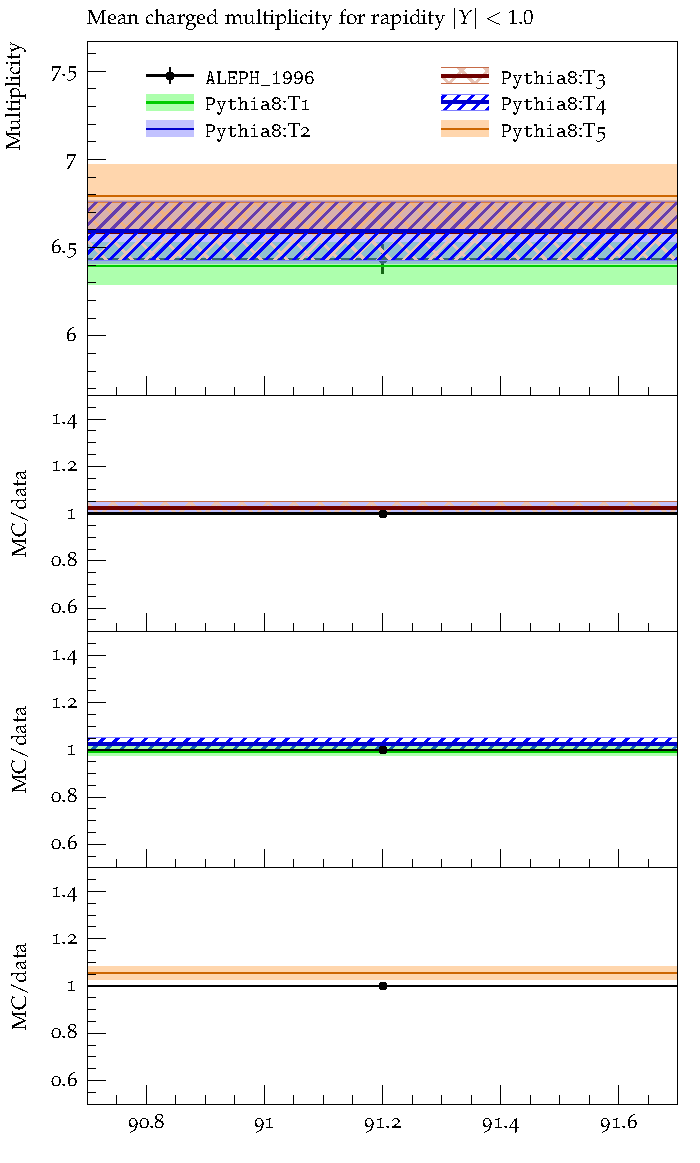
\includegraphics[width=8cm, height=9cm]{ALEPH_1996/d21-x01-y01.pdf}
 \hfill
  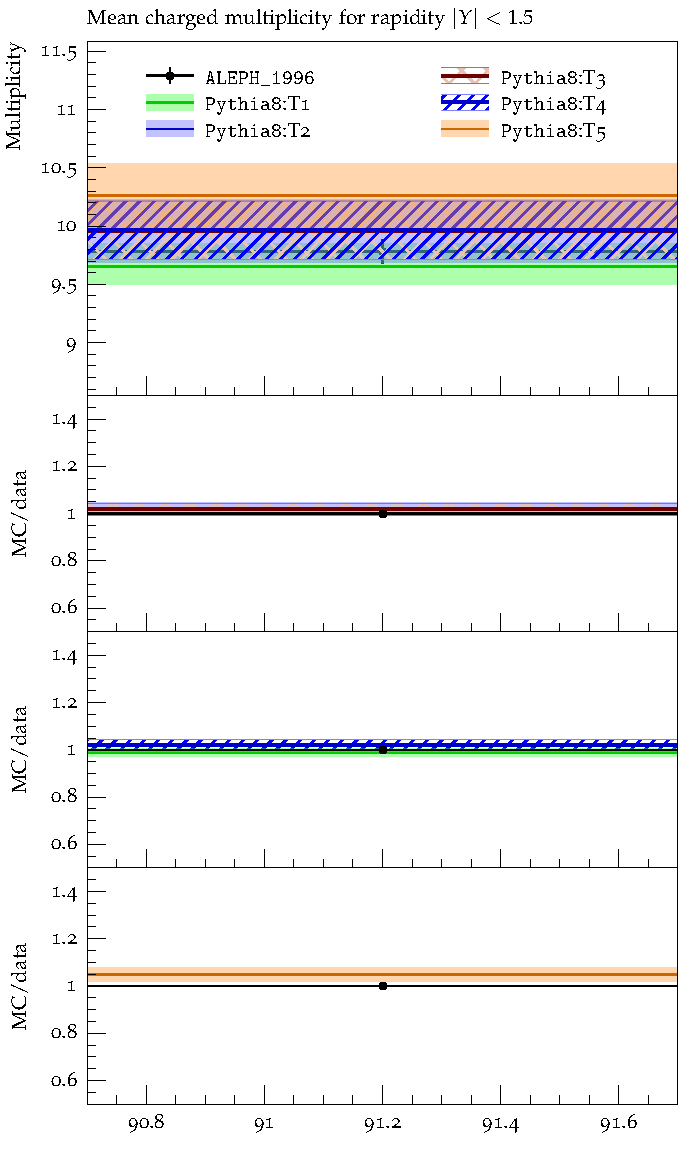
\includegraphics[width=8cm, height=9cm]{ALEPH_1996/d22-x01-y01.pdf}
  \caption{Mean charged multiplicity (left top), for $|Y| < 0.5$ (right top), $|Y| < 1$ (left bottom)
  and $|Y| < 1.5$ (right bottom). Data taken from \cite{Barate:1996fi}.}
  \label{Fig-2}
 \end{figure} 
 
 
\begin{figure}[btp]
 \centering
 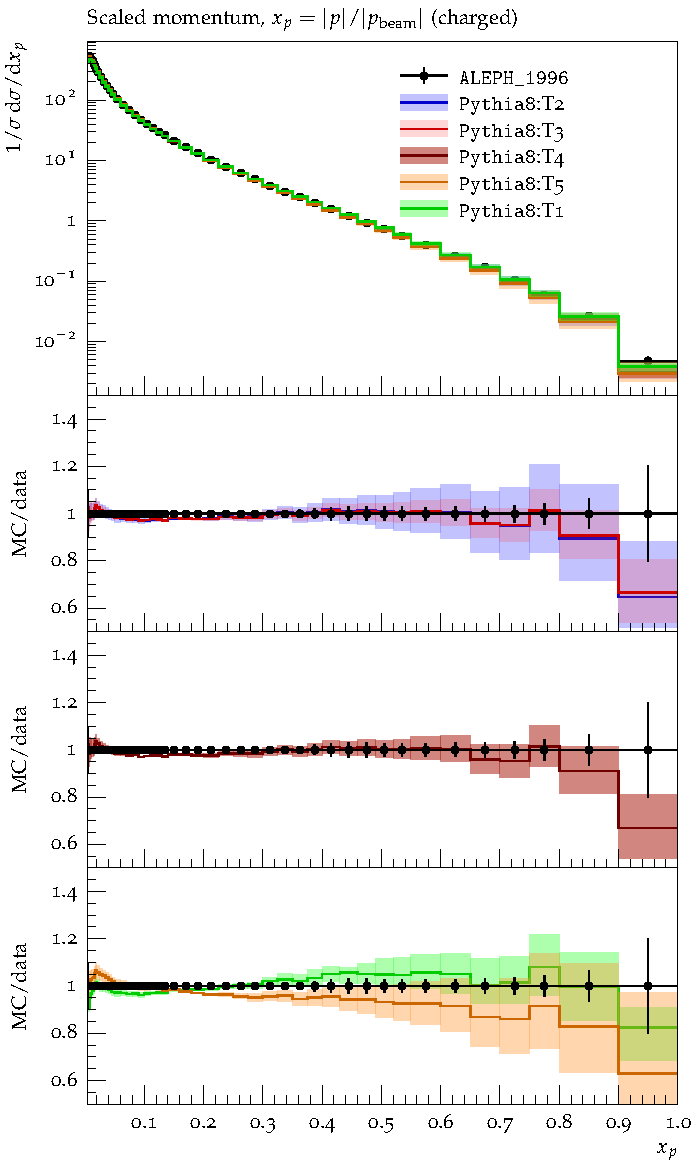
\includegraphics[width=8cm, height=9cm]{ALEPH_1996/d09-x01-y01.pdf}
 \hfill
  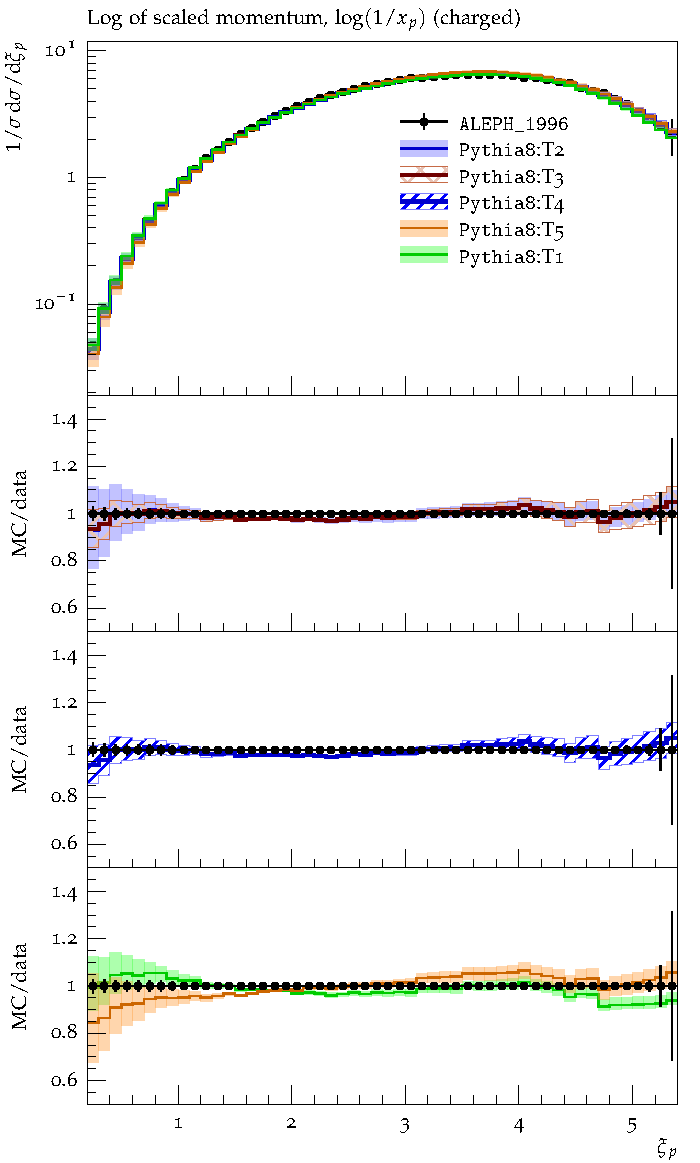
\includegraphics[width=8cm, height=9cm]{ALEPH_1996/d17-x01-y01.pdf}
  \vfill
     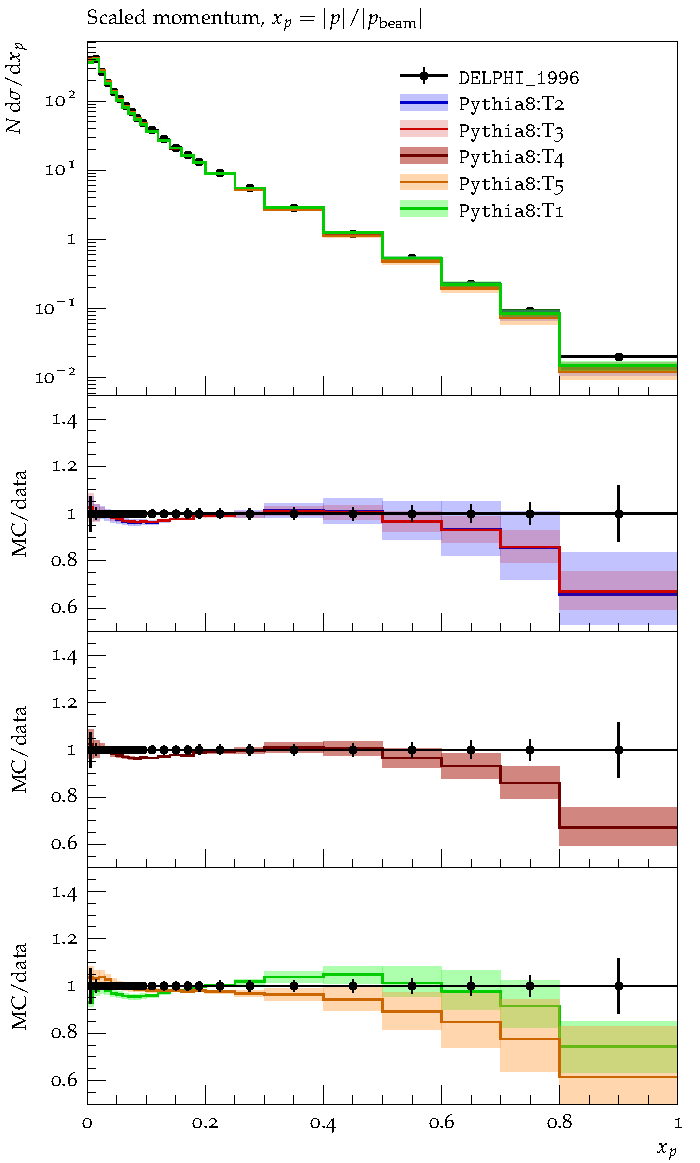
\includegraphics[width=8cm, height=9cm]{DELPHI_1996/d07-x01-y01.pdf}
 \hfill
  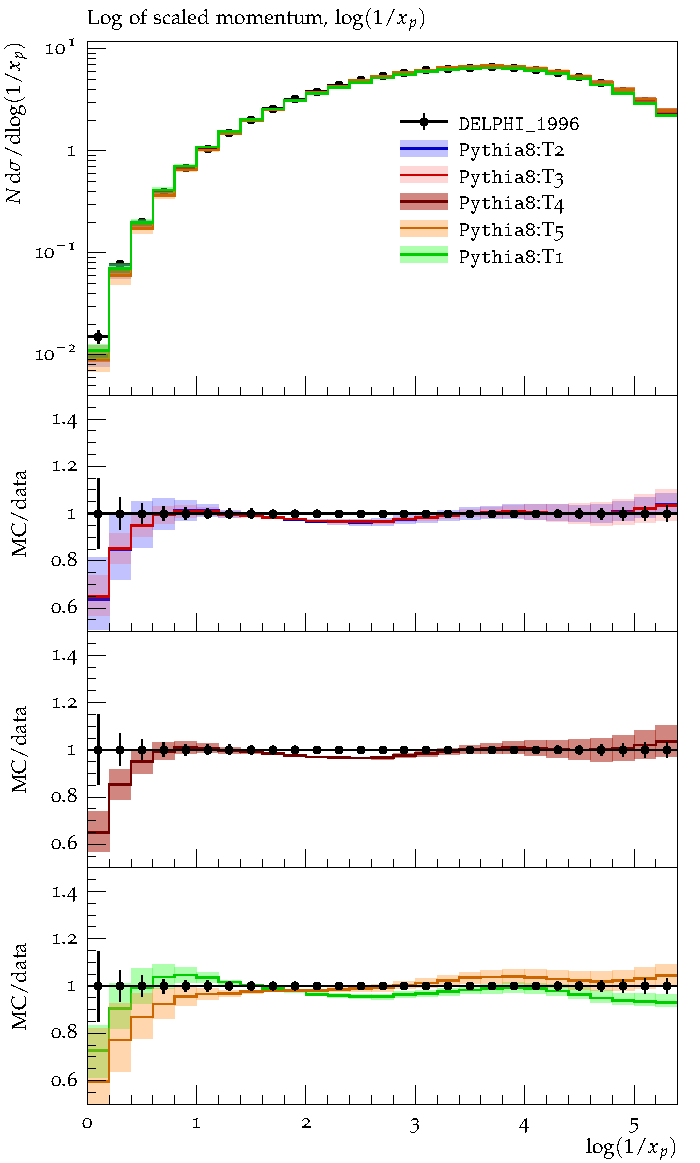
\includegraphics[width=8cm, height=9cm]{DELPHI_1996/d08-x01-y01.pdf}
  \caption{Scaled momentum distribution for charged particles (top) and all particles (bottom). Data
  from \cite{Barate:1996fi} and \cite{Abreu:1996na}.}
  \label{Fig-3}
 \end{figure}
 
 
 
  \begin{figure}[!h]
  \centering
   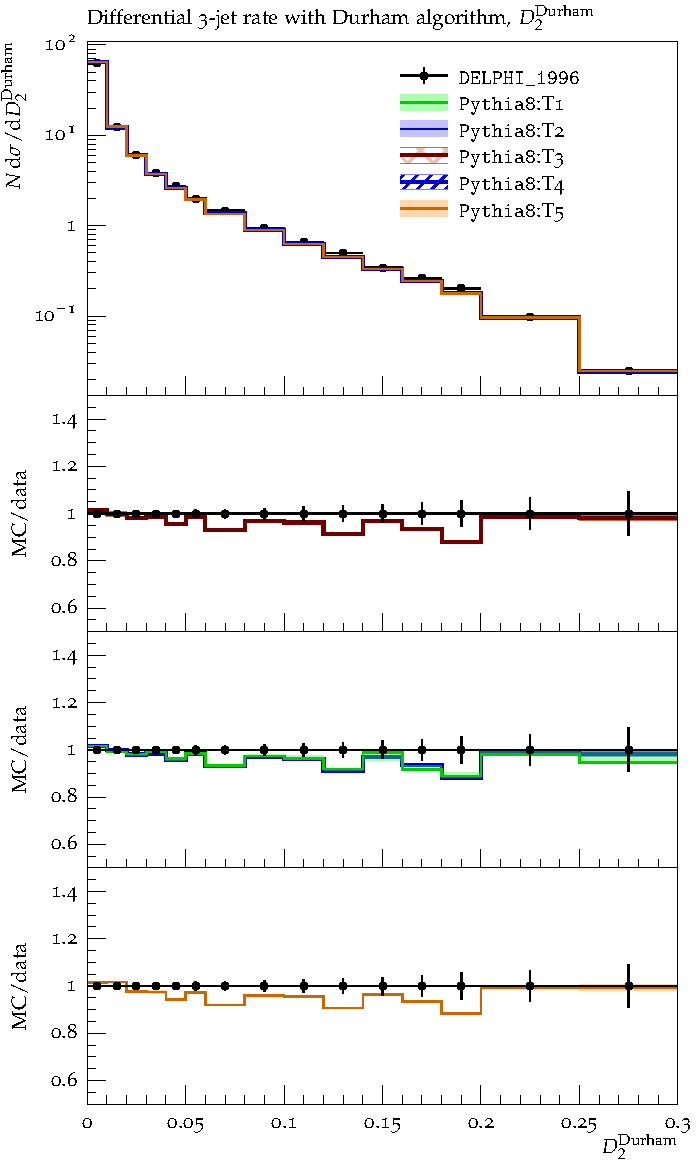
\includegraphics[width=8cm, height=9cm]{DELPHI_1996/d27-x01-y01.pdf}
 \hfill
  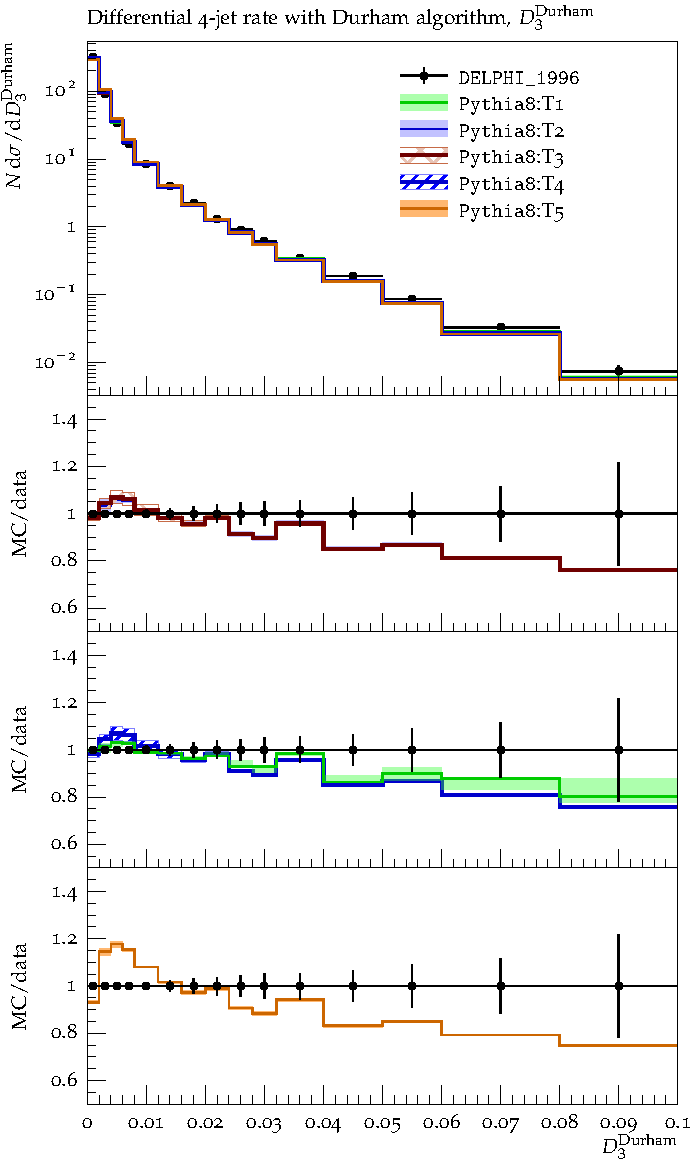
\includegraphics[width=8cm, height=9cm]{DELPHI_1996/d29-x01-y01.pdf}
  \caption{Differential $3$- (left) and $4$- (right) jet rate. Data from \cite{Abreu:1996na}. }
  \label{Fig-4}
 \end{figure}

 
 \begin{figure}[btp]
 \centering
 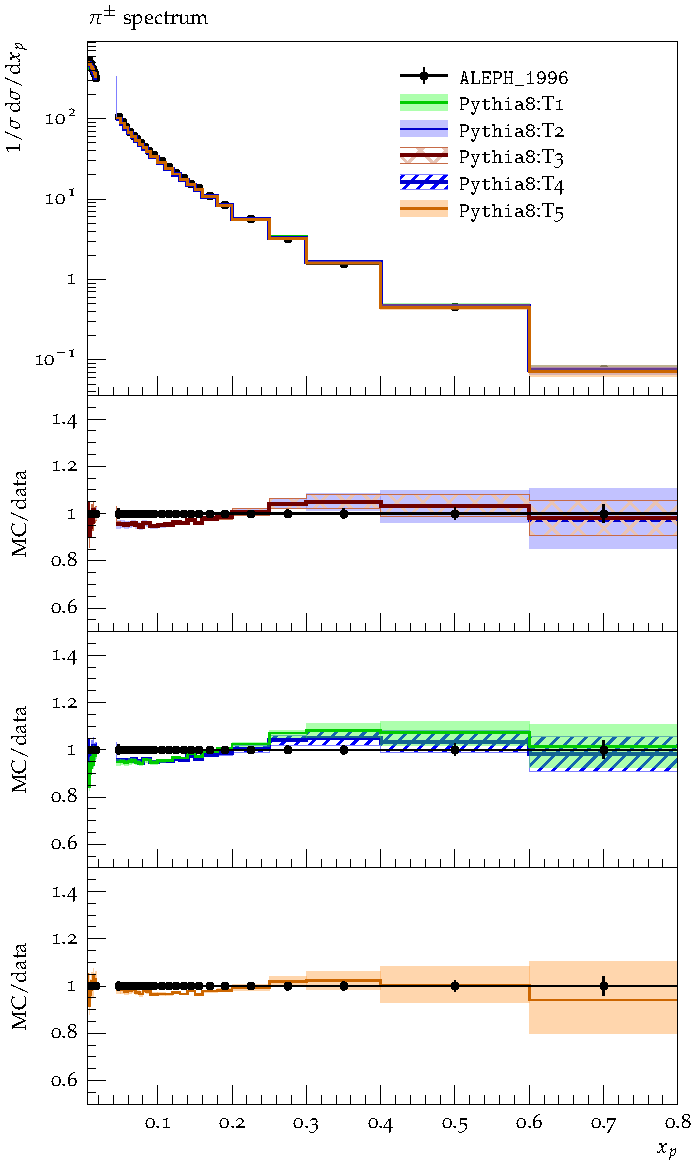
\includegraphics[width=8cm, height=9cm]{ALEPH_1996/d25-x01-y01.pdf}
 \hfill
  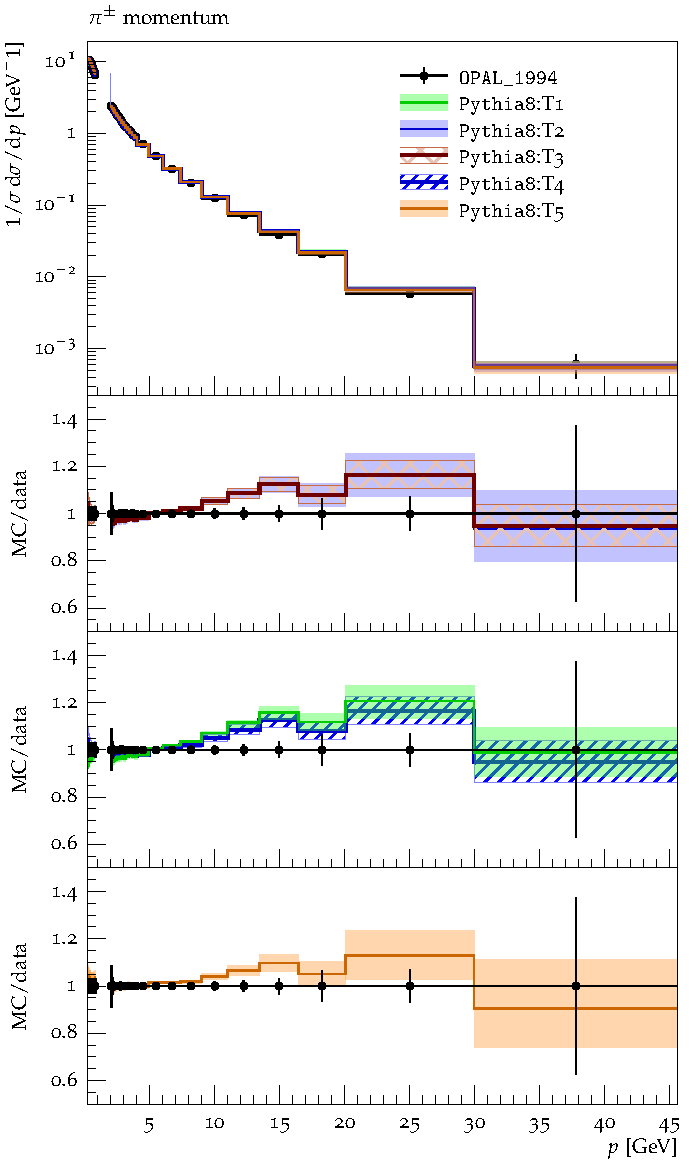
\includegraphics[width=8cm, height=9cm]{OPAL_1994/d01-x01-y01.pdf}
  \caption{Charged pion momentum distribution. Data from \cite{Barate:1996fi, Akers:1994ez}.}
  \label{Fig-5}
 \end{figure}
 
  \begin{figure}[btp]
 \centering
 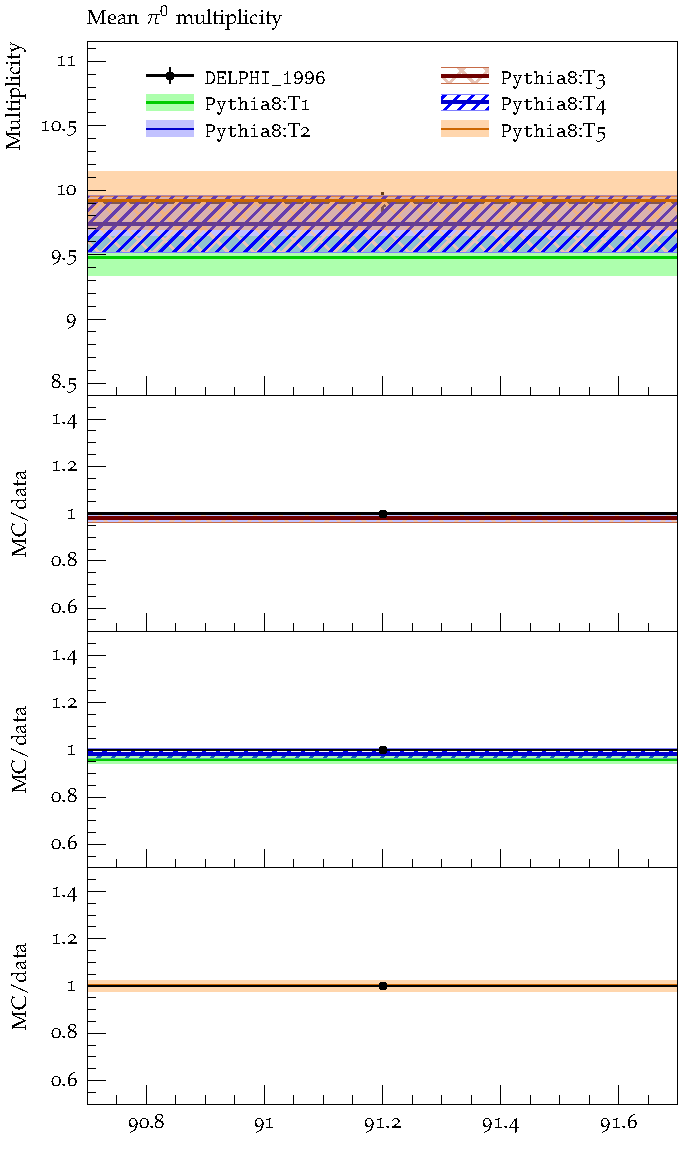
\includegraphics[width=8cm, height=9cm]{DELPHI_1996/d36-x01-y02.pdf}
 \hfill
  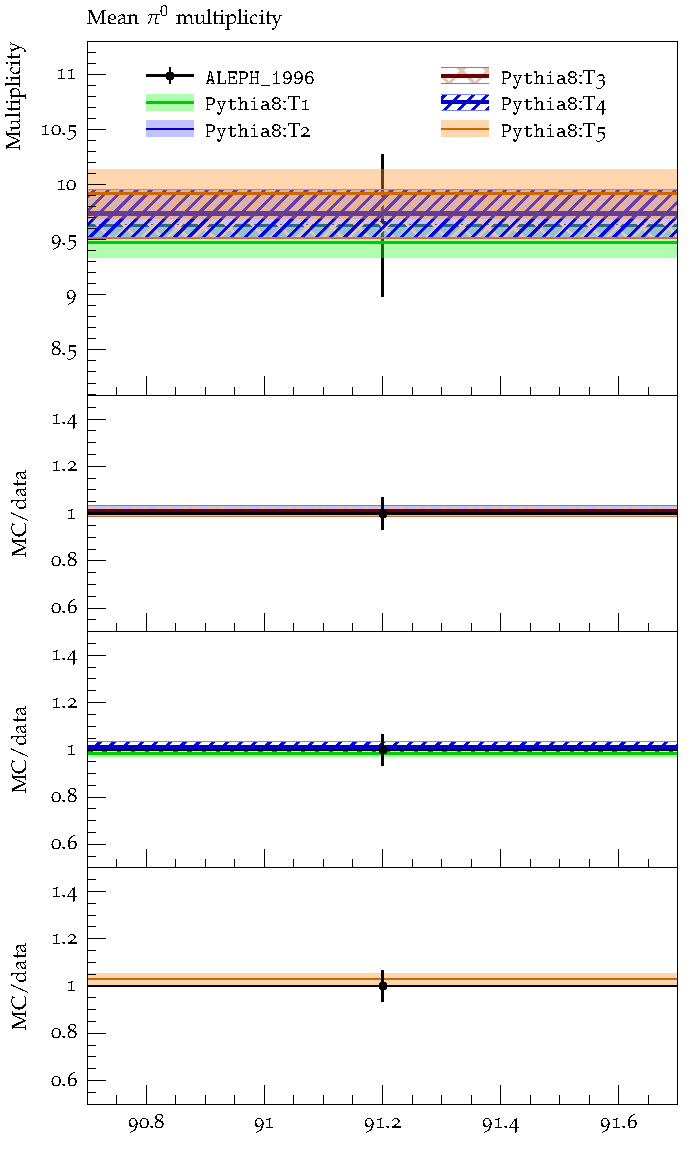
\includegraphics[width=8cm, height=9cm]{ALEPH_1996/d44-x01-y02.pdf}
  \caption{Mean $\pi^0$ multiplicity. Data from \cite{Barate:1996fi, Abreu:1996na}.}
  \label{Fig-6}
 \end{figure}
 
   \begin{figure}[btp]
 \centering
 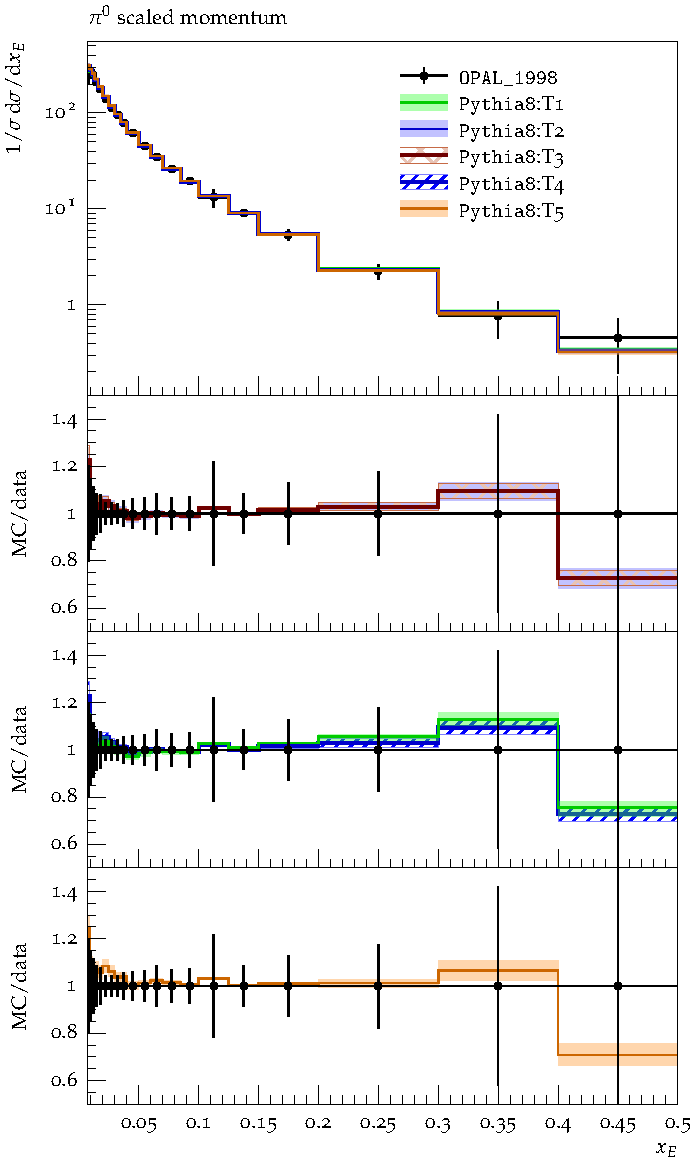
\includegraphics[width=8cm, height=9cm]{OPAL_1998/d04-x01-y01.pdf}
 \hfill
  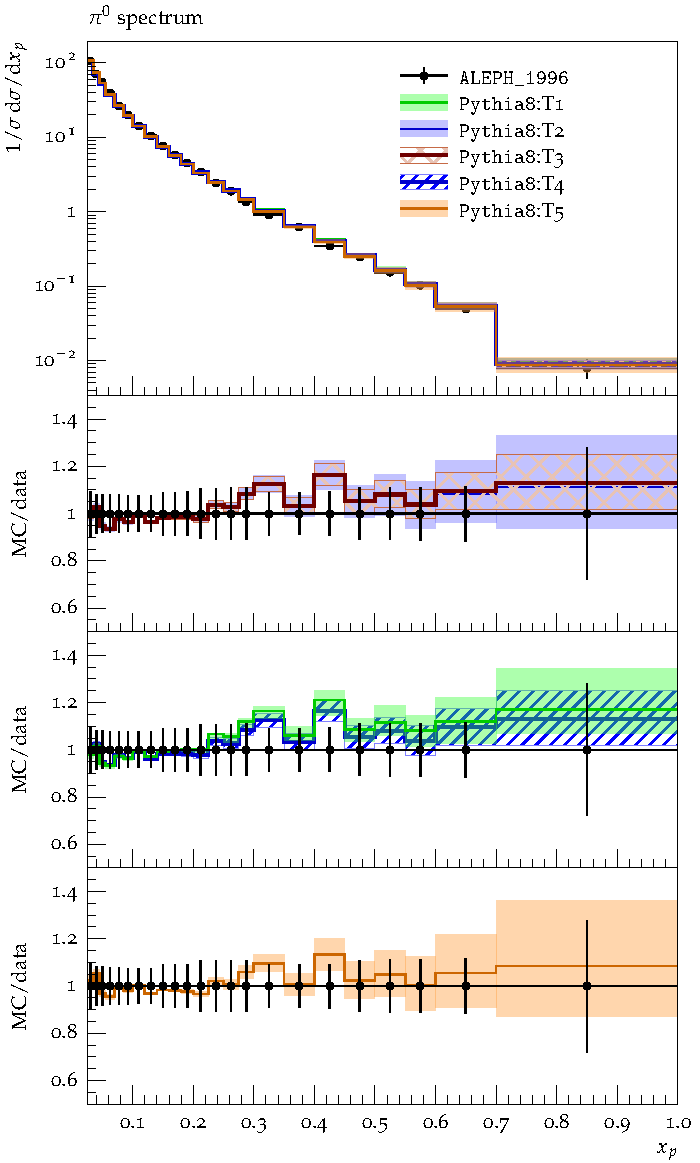
\includegraphics[width=8cm, height=9cm]{ALEPH_1996/d29-x01-y01.pdf}
  \caption{$\pi^0$ momentum distribution. Data from \cite{Barate:1996fi, Ackerstaff:1998ap}.}
  \label{Fig-7}
 \end{figure}

 
 \begin{figure}[btp]
  \centering
   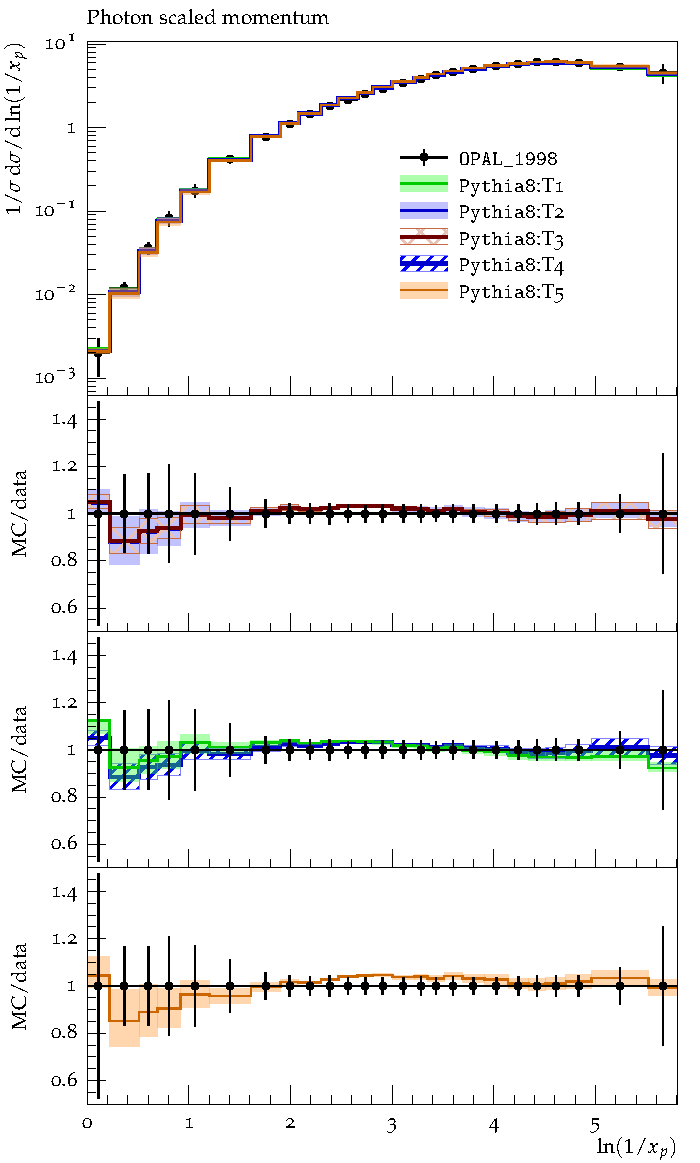
\includegraphics[width=8cm, height=9cm]{OPAL_1998/d03-x01-y01.pdf}
 \hfill
  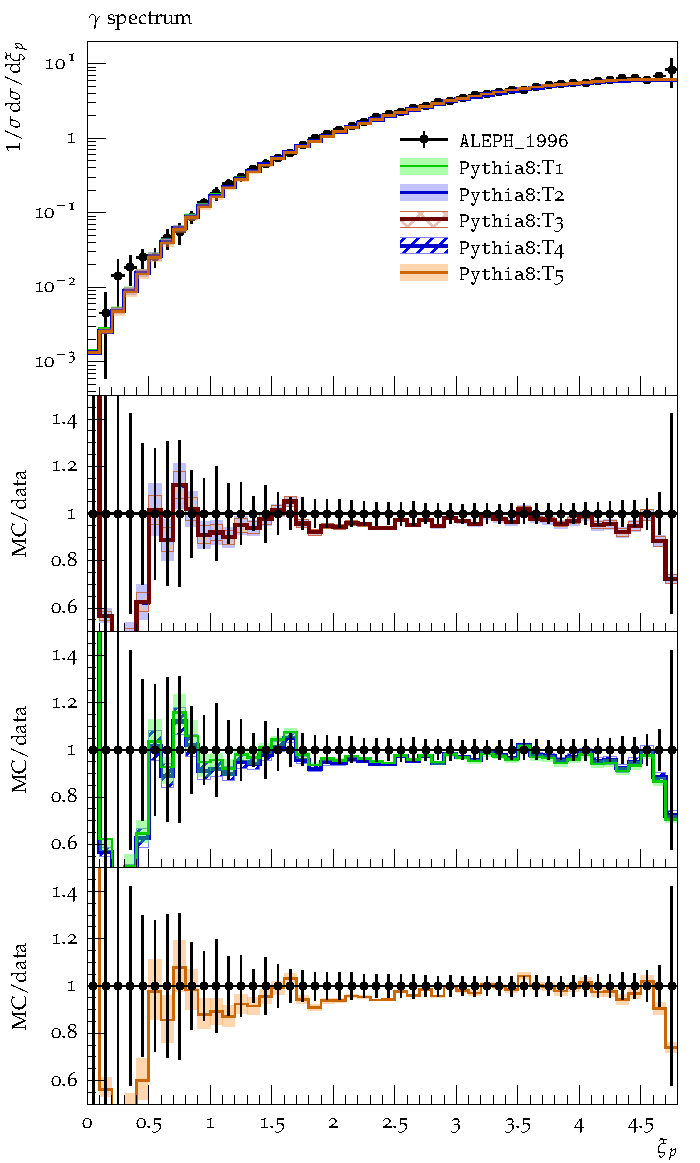
\includegraphics[width=8cm, height=9cm]{ALEPH_1996/d28-x01-y01.pdf}
  \caption{$\gamma$ spectrum. Data is taken from \cite{Barate:1996fi, Ackerstaff:1998ap}.}
  \label{Fig-8}
 \end{figure}



\clearpage
\appendix
\section{Observables and their weights}
 \begin{table}[!h]
  \begin{center}
   \begin{tabular}{l|l}
    \hline 
    \hline
    Observable  \hspace{3cm} &  \hspace{1cm} Associated Weight \\ \hline
    $\pi^0$ spectrum & \hspace{3cm} $30.0$ \\ \hline
    $\pi^\pm$ spectrum & \hspace{3cm} $30.0$ \\ \hline
    $\rho$ spectrum &\hspace{3cm} $1.0$ \\ \hline
    $K^{*0,\pm}$ spectrum &\hspace{3cm} $1.0$ \\ \hline
    $\omega$ spectrum & \hspace{3cm} $1.0$ \\ \hline
    $K^0$ spectrum & \hspace{3cm} $1.0$ \\ \hline
    $\eta'$ spectrum & \hspace{3cm} $1.0$ \\ \hline
    $\gamma$ spectrum & \hspace{3cm} $30.0$ \\ \hline
    $\eta$ spectrum & \hspace{3cm} $1.0$ \\ \hline \hline
   \end{tabular}
  \end{center}
  \caption{Identified photon and meson spectra and their weights.}
  \label{Tab1}
 \end{table}
 
 \begin{table}[tbp]
  \begin{center}
   \begin{tabular}{l|l}
    \hline 
    \hline
    Observable  \hspace{3cm} &  \hspace{1cm} Associated Weight \\ \hline
    Mean charged multiplicity & \hspace{3cm} $50.0$ \\ \hline
    Mean $\pi^0, \pi^\pm$ multiplicity & \hspace{3cm} $50.0$ \\ \hline
    Mean $\rho$ multiplicity &\hspace{3cm} $1.0$ \\ \hline
    Mean $K^{*0}$ multiplicity &\hspace{3cm} $1.0$ \\ \hline
    Mean $\omega$ multiplicity & \hspace{3cm} $1.0$ \\ \hline
    Mean $K^0$ multiplicity & \hspace{3cm} $1.0$ \\ \hline
    Mean $K_S + K_L$ multiplicity & \hspace{3cm} $1.0$ \\ \hline
    Mean $\eta'$ multiplicity & \hspace{3cm} $1.0$ \\ \hline
    Mean $\eta$ multiplicity & \hspace{3cm} $1.0$ \\ \hline \hline
   \end{tabular}
  \end{center}
  \caption{Mean particle multiplicities and their weights.}
  \label{Tab2}
 \end{table}

   \begin{table}[tbp]
  \begin{center}
   \begin{tabular}{l|l}
    \hline 
    \hline
    Observable  \hspace{3cm} &  \hspace{1cm} Associated Weight \\ \hline
    Differential $3$-jet rate with Durham algorithm & \hspace{3cm} $2.0$ \\ \hline
    Differential $3$-jet rate with Jade algorithm & \hspace{3cm} $2.0$ \\ \hline
    Differential $4$-jet rate with Durham algorithm &\hspace{3cm} $2.0$ \\ \hline
    Differential $4$-jet rate with Jade algorithm &\hspace{3cm} $2.0$ \\ \hline
    Differential $5$-jet rate with Durham algorithm & \hspace{3cm} $1.0$ \\ \hline
    Differential $5$-jet rate with Jade algorithm & \hspace{3cm} $1.0$ \\ \hline \hline
   \end{tabular}
  \end{center}
  \caption{Jet rates and their weights}
  \label{Tab3}
 \end{table}
 
  \begin{table}[tbp]
\begin{center}
\begin{tabular}{l|l}
\hline \hline 
Observable \hspace{1cm} &  Associated Weight \\ \hline
In(out-)-plane $p_\bot$ in GeV w.r.t. (thrust) sphericity axes & \hspace{1cm} $1.0$ \\ \hline 
Mean out-of-plane $p_\bot$ in GeV w.r.t. thrust axis vs. $x_p$ & \hspace{1cm} $1.0$ \\ \hline
Scaled momentum $x_p=|p|/|p_\text{beam}|$ & \hspace{1cm} $1.0$ \\ \hline
Log of scaled momentum, $\log(1/x_p)$ & \hspace{1cm} $1.0$ \\ \hline
Energy-energy correlation, EEC & \hspace{1cm} $1.0$ \\ \hline
Sphericity, $S$ & \hspace{1cm} $1.0$ \\ \hline
Aplanarity, $A$ & \hspace{1cm} $1.0$ \\ \hline
Planarity, $P$ & \hspace{1cm} $1.0$ \\ \hline
$D$ parameter & \hspace{1cm} $1.0$ \\ \hline
$C$ parameter & \hspace{1cm} $1.0$ \\ \hline
1-Thrust & \hspace{1cm} $1.0$ \\ \hline
Thrust major, $M$ & \hspace{1cm} $1.0$ \\ \hline
Thrust minor, $m$ & \hspace{1cm} $1.0$\\ \hline
Oblateness, $O=M-m$ &  \hspace{1cm} $1.0$ \\ \hline
Charged multiplicity distribution  & \hspace{1cm} $1.0$ \\ \hline
Mean charged multiplicity & \hspace{1cm} $1.0$ \\ \hline
\hline
\end{tabular}
\end{center}
\caption{Event shapes and the associated weights.}
\label{Tab4}
 \end{table}

 \begin{table}[tbp]
  \begin{center}
   \begin{tabular}{l|l}
    \hline 
    \hline
    Observable  \hspace{3cm} &  \hspace{1cm} Associated Weight \\ \hline
    $\pi^0$ spectrum & \hspace{3cm} $30.0$ \\ \hline
    $\pi^\pm$ spectrum & \hspace{3cm} $30.0$ \\ \hline
    Charged multiplicity &\hspace{3cm} $1.0$ \\ \hline
    mean charged multiplicity &\hspace{3cm} $50.0$ \\ \hline
    mean $\pi^{0,\pm}$ multiplicities & \hspace{3cm} $50.0$ \\ \hline
    Scaled momentum (charged) & \hspace{3cm} $30.0$ \\ \hline
    Scaled momentum & \hspace{3cm} $30.0$ \\ \hline
    $\gamma$ spectrum & \hspace{3cm} $30.0$ \\ \hline
    $\eta$ spectrum & \hspace{3cm} $1.0$ \\ \hline \hline
   \end{tabular}
  \end{center}
  \caption{observables included in \texttt{T3} tune.}
  \label{Tab5}
\end{table}

 \begin{table}[tbp]
  \begin{center}
   \begin{tabular}{l|l}
    \hline 
    \hline
    Observable  \hspace{3cm} &  \hspace{1cm} Associated Weight \\ \hline
    $\pi^0$ spectrum & \hspace{3cm} $30.0$ \\ \hline
    $\pi^\pm$ spectrum & \hspace{3cm} $30.0$ \\ \hline
    mean $\pi^{0,\pm}$ multiplicities & \hspace{3cm} $50.0$ \\ \hline
    Scaled momentum (charged) & \hspace{3cm} $30.0$ \\ \hline
    Scaled momentum & \hspace{3cm} $30.0$ \\ \hline
    $\gamma$ spectrum & \hspace{3cm} $30.0$ \\ \hline
    $\eta$ spectrum & \hspace{3cm} $1.0$ \\ \hline \hline
   \end{tabular}
  \end{center}
  \caption{observables included in \texttt{T4} tune.}
  \label{Tab6}
\end{table}

 \begin{table}[tbp]
  \begin{center}
   \begin{tabular}{l|l}
    \hline 
    \hline
    Observable  \hspace{3cm} &  \hspace{1cm} Associated Weight \\ \hline
    $\pi^0$ spectrum & \hspace{3cm} $30.0$ \\ \hline
    $\pi^\pm$ spectrum & \hspace{3cm} $30.0$ \\ \hline
    $\gamma$ spectrum & \hspace{3cm} $30.0$ \\ \hline
    $\eta$ spectrum & \hspace{3cm} $1.0$ \\ \hline \hline
   \end{tabular}
  \end{center}
  \caption{observables included in \texttt{T5} tune.}
  \label{Tab7}
\end{table}
\clearpage 
\begin{thebibliography}{99}
\bibitem{Bertone:2004pz}
  G.~Bertone, D.~Hooper and J.~Silk,
  ``Particle dark matter: Evidence, candidates and constraints,''
  Phys.\ Rept.\  {\bf 405} (2005) 279
  doi:10.1016/j.physrep.2004.08.031
  [hep-ph/0404175].
  
 \bibitem{Barate:1996fi}
  R.~Barate {\it et al.} [ALEPH Collaboration],
  ``Studies of quantum chromodynamics with the ALEPH detector,''
  Phys.\ Rept.\  {\bf 294} (1998) 1.
  doi:10.1016/S0370-1573(97)00045-8
  
  \bibitem{Heister:2001jg}
  A.~Heister {\it et al.} [ALEPH Collaboration],
  ``Study of the fragmentation of b quarks into B mesons at the Z peak,''
  Phys.\ Lett.\ B {\bf 512} (2001) 30
  doi:10.1016/S0370-2693(01)00690-6
  [hep-ex/0106051].
  
  \bibitem{Heister:2001kp}
  A.~Heister {\it et al.} [ALEPH Collaboration],
  ``Inclusive production of the omega and eta mesons in Z decays, and the muonic branching ratio of the omega,''
  Phys.\ Lett.\ B {\bf 528} (2002) 19
  doi:10.1016/S0370-2693(02)01220-0
  [hep-ex/0201012].
  
  \bibitem{Abreu:1996na}
  P.~Abreu {\it et al.} [DELPHI Collaboration],
  ``Tuning and test of fragmentation models based on identified particles and precision event shape data,''
  Z.\ Phys.\ C {\bf 73} (1996) 11.
  doi:10.1007/s002880050295
  
  \bibitem{Abreu:1998nn}
  P.~Abreu {\it et al.} [DELPHI Collaboration],
  ``Measurement of inclusive rho0, f(0)(980), f(2)(1270), K*0(2)(1430) and f-prime(2)(1525) production in Z0 decays,''
  Phys.\ Lett.\ B {\bf 449} (1999) 364.
  doi:10.1016/S0370-2693(99)00105-7
  
  \bibitem{DELPHI_2002}
  Study of the b-quark fragmentation function at LEP 1, 
  DELPHI note 2002-069-CONF-603 (ICHEP 2002)
  
  \bibitem{Akers:1994ez}
  R.~Akers {\it et al.} [OPAL Collaboration],
  ``Measurement of the production rates of charged hadrons in e+ e- annihilation at the Z0,''
  Z.\ Phys.\ C {\bf 63} (1994) 181.
  doi:10.1007/BF01411010
  
  \bibitem{Ackerstaff:1998ap}
  K.~Ackerstaff {\it et al.} [OPAL Collaboration],
  ``Photon and light meson production in hadronic Z0 decays,''
  Eur.\ Phys.\ J.\ C {\bf 5} (1998) 411
  doi:10.1007/s100520050286
  [hep-ex/9805011].
  
  \bibitem{Abbiendi:2000cv}
  G.~Abbiendi {\it et al.} [OPAL Collaboration],
  ``Multiplicities of pi0, eta, K0 and of charged particles in quark and gluon jets,''
  Eur.\ Phys.\ J.\ C {\bf 17} (2000) 373
  doi:10.1007/s100520000505
  [hep-ex/0007017].
  
  \bibitem{Abe:1996zi}
  K.~Abe {\it et al.} [SLD Collaboration],
  ``Measurement of the charged multiplicities in b, c and light quark events from Z0 decays,''
  Phys.\ Lett.\ B {\bf 386} (1996) 475
  doi:10.1016/0370-2693(96)01025-8
  [hep-ex/9608008].
  
  \bibitem{Abe:1998zs}
  K.~Abe {\it et al.} [SLD Collaboration],
  ``Production of pi+, K+, K0, K*0, phi, p and Lambda0 in hadronic Z0 decays,''
  Phys.\ Rev.\ D {\bf 59} (1999) 052001
  doi:10.1103/PhysRevD.59.052001
  [hep-ex/9805029].
  
  \bibitem{Abe:2002iq}
  K.~Abe {\it et al.} [SLD Collaboration],
  ``Measurement of the b quark fragmentation function in Z0 decays,''
  Phys.\ Rev.\ D {\bf 65} (2002) 092006
   Erratum: [Phys.\ Rev.\ D {\bf 66} (2002) 079905]
  doi:10.1103/PhysRevD.66.079905, 10.1103/PhysRevD.65.092006
  [hep-ex/0202031].
  
  \bibitem{Giele:2007di}
  W.~T.~Giele, D.~A.~Kosower and P.~Z.~Skands,
  %``A simple shower and matching algorithm,''
  Phys.\ Rev.\ D {\bf 78} (2008) 014026
  doi:10.1103/PhysRevD.78.014026
  [arXiv:0707.3652 [hep-ph]].
  %%CITATION = doi:10.1103/PhysRevD.78.014026;%%
  
  \bibitem{Buckley:2011ms}
  A.~Buckley {\it et al.},
  ``General-purpose event generators for LHC physics,''
  Phys.\ Rept.\  {\bf 504} (2011) 145
  doi:10.1016/j.physrep.2011.03.005
  [arXiv:1101.2599 [hep-ph]].
  
  \bibitem{Buckley:2009bj}
  A.~Buckley, H.~Hoeth, H.~Lacker, H.~Schulz and J.~E.~von Seggern,
  ``Systematic event generator tuning for the LHC,''
  Eur.\ Phys.\ J.\ C {\bf 65} (2010) 331
  doi:10.1140/epjc/s10052-009-1196-7
  [arXiv:0907.2973 [hep-ph]].
  
  \bibitem{Buckley:2010ar}
  A.~Buckley, J.~Butterworth, L.~Lonnblad, D.~Grellscheid, H.~Hoeth, J.~Monk, H.~Schulz and F.~Siegert,
  ``Rivet user manual,''
  Comput.\ Phys.\ Commun.\  {\bf 184} (2013) 2803
  doi:10.1016/j.cpc.2013.05.021
  [arXiv:1003.0694 [hep-ph]].
  
  \bibitem{Sjostrand:2006za}
  T.~Sjostrand, S.~Mrenna and P.~Z.~Skands,
  ``PYTHIA 6.4 Physics and Manual,''
  JHEP {\bf 0605} (2006) 026
  doi:10.1088/1126-6708/2006/05/026
  [hep-ph/0603175].
  
  \bibitem{Sjostrand:2007gs}
  T.~Sjostrand, S.~Mrenna and P.~Z.~Skands,
  ``A Brief Introduction to PYTHIA 8.1,''
  Comput.\ Phys.\ Commun.\  {\bf 178} (2008) 852
  doi:10.1016/j.cpc.2008.01.036
  [arXiv:0710.3820 [hep-ph]].
  
  \bibitem{Sjostrand:2014zea}
  T.~Sjöstrand {\it et al.},
  ``An Introduction to PYTHIA 8.2,''
  Comput.\ Phys.\ Commun.\  {\bf 191} (2015) 159
  doi:10.1016/j.cpc.2015.01.024
  [arXiv:1410.3012 [hep-ph]].
  
  \bibitem{Skands:2014pea}
  P.~Skands, S.~Carrazza and J.~Rojo,
  ``Tuning PYTHIA 8.1: the Monash 2013 Tune,''
  Eur.\ Phys.\ J.\ C {\bf 74} (2014) no.8,  3024
  doi:10.1140/epjc/s10052-014-3024-y
  [arXiv:1404.5630 [hep-ph]].
  
  \bibitem{Cembranos:2013cfa}
  J.~A.~R.~Cembranos, A.~de la Cruz-Dombriz, V.~Gammaldi, R.~A.~Lineros and A.~L.~Maroto,
  ``Reliability of Monte Carlo event generators for gamma ray dark matter searches,''
  JHEP {\bf 1309} (2013) 077
  doi:10.1007/JHEP09(2013)077
  [arXiv:1305.2124 [hep-ph]].

    \bibitem{Bowler:1981sb}
  M.~G.~Bowler,
  ``e+ e- Production of Heavy Quarks in the String Model,''
  Z.\ Phys.\ C {\bf 11} (1981) 169.
  doi:10.1007/BF01574001
 
\end{thebibliography}

\end{document}          
